% paper.tex
%
% LaTeX template for creating an MNRAS paper
%
% v3.0 released 14 May 2015
% (version numbers match those of mnras.cls)
%
% Copyright (C) Royal Astronomical Society 2015
% Authors:
% Keith T. Smith (Royal Astronomical Society)

% Change log
%
% v3.0 May 2015
%    Renamed to match the new package name
%    Version number matches mnras.cls
%    A few minor tweaks to wording
% v1.0 September 2013
%    Beta testing only - never publicly released
%    First version: a simple (ish) template for creating an MNRAS paper

%%%%%%%%%%%%%%%%%%%%%%%%%%%%%%%%%%%%%%%%%%%%%%%%%%
% Basic setup. Most papers should leave these options alone.
\documentclass[a4paper,fleqn,usenatbib]{mnras}

% MNRAS is set in Times font. If you don't have this installed (most LaTeX
% installations will be fine) or prefer the old Computer Modern fonts, comment
% out the following line
\usepackage{newtxtext,newtxmath}
% Depending on your LaTeX fonts installation, you might get better results with 
% one of these:
%\usepackage{mathptmx}
%\usepackage{txfonts}

% Use vector fonts, so it zooms properly in on-screen viewing software
% Don't change these lines unless you know what you are doing
\usepackage[T1]{fontenc}
\usepackage{ae,aecompl}


%%%%% AUTHORS - PLACE YOUR OWN PACKAGES HERE %%%%%

% Only include extra packages if you really need them. Common packages are:
\usepackage{graphicx}	% Including figure files
\usepackage{amsmath}	% Advanced maths commands
\usepackage{amssymb}	% Extra maths symbols
\usepackage{mathtools}
\usepackage{hyperref}
%%%%%%%%%%%%%%%%%%%%%%%%%%%%%%%%%%%%%%%%%%%%%%%%%%

%%%%% AUTHORS - PLACE YOUR OWN COMMANDS HERE %%%%%

\newcommand{\fesc}{\ifmmode{f_{\rm esc}}\else{$f_{\rm esc}$}\fi}
\newcommand{\fescs}{\ifmmode{f_{\rm esc}^\star}\else{$f_{\rm esc}^\star$}\fi}
\newcommand{\kms}{\ifmmode{{\;\rm km~s^{-1}}}\else{km~s$^{-1}$}\fi}
\newcommand{\fgas}{\ifmmode{{f_{\rm gas}}}\else{$f_{\rm gas}$}\fi}
\newcommand{\cubecm}{\ifmmode{{\rm cm^{-3}}}\else{cm$^{-3}$}\fi}
\newcommand{\ztwo}{\ifmmode{{\rm [Z_2/H]}}\else{[Z$_2$/H]}\fi}
\newcommand{\zthree}{\ifmmode{{\rm [Z_3/H]}}\else{[Z$_3$/H]}\fi}
\newcommand{\lsim}{\lower0.3em\hbox{$\,\buildrel <\over\sim\,$}}
\newcommand{\gsim}{\lower0.3em\hbox{$\,\buildrel >\over\sim\,$}}
\newcommand{\li}{\noindent$\bullet$\quad}
\newcommand{\lli}{$\bullet$\quad}
\newcommand{\lcdm}{$\Lambda$CDM}
\newcommand{\flux}{erg s$^{-1}$ cm$^{-2}$ Hz$^{-1}$}
\newcommand{\emis}{erg s$^{-1}$ cm$^{-2}$ Hz$^{-1}$ sr$^{-1}$}
\newcommand{\sfr}{\ifmmode{\textrm{M}_\odot \,\textrm{yr}^{-1} \,\textrm{Mpc}^{-3}}\else{M$_\odot$ yr$^{-1}$ Mpc$^{-3}$}\fi}
\newcommand{\hsfr}{\ifmmode{\textrm{M}_\odot\, \textrm{yr}^{-1}}\else{M$_\odot$ yr$^{-1}$}\fi}
\newcommand{\ssfr}{Gyr$^{-1}$}
\newcommand{\arp}{$a_{\rm rp}$}
\newcommand{\agrav}{$a_{\rm grav}$}
\newcommand{\eavg}{\ifmmode{\langle E_\gamma \rangle}\else{$\langle E_\gamma \rangle$}\fi}
\newcommand{\hst}{{\it HST}}
\newcommand{\enzo}{{\sc enzo}}
\newcommand{\yt}{{\sc yt}}
\newcommand{\moray}{{\sc enzo+moray}}
\newcommand{\Ms}{\ifmmode{M_\odot}\else{$M_\odot$}\fi}
\newcommand{\vrms}{\ifmmode{v_{\rm rms}}\else{$v_{\rm rms}$}\fi}
\newcommand{\mmin}{M$_{min}$}
\newcommand{\hh}{H$_2$}
\newcommand{\Ol}{$\Omega_\Lambda$}
\newcommand{\Om}{$\Omega_M$}
\newcommand{\Ob}{$\Omega_b$}
\newcommand{\theat}{$t_{\rm{heat}}$}
\newcommand{\tcool}{$t_{\rm{cool}}$}
\newcommand{\rcool}{$r_{\rm{cool}}$}
\newcommand{\tcross}{$t_{\rm{cross}}$}
\newcommand{\tdyn}{$t_{\rm{dyn}}$}
\newcommand{\tkh}{$t_{\rm{KH}}$}
\newcommand{\tH}{$t_{\rm{H}}$}
\newcommand{\tvir}{\ifmmode{T_{\rm{vir}}}\else{$T_{\rm{vir}}$}\fi}
\newcommand{\mvir}{\ifmmode{M_{\rm{vir}}}\else{$M_{\rm{vir}}$}\fi}
\newcommand{\rvir}{\ifmmode{r_{\rm{vir}}}\else{$r_{\rm{vir}}$}\fi}
\newcommand{\rr}{$r_{200}$}
\newcommand{\lya}{Ly$\alpha$}
\newcommand{\jj}{\ifmmode{J_{21}}\else{$J_{21}$}\fi}
\newcommand{\flw}{\ifmmode{F_{LW}}\else{$F_{LW}$}\fi}
\newcommand{\kph}{\ifmmode{k_{\rm ph}}\else{$k_{\rm ph}$}\fi}
\newcommand{\tv}{$\langle T \rangle_{\rm v}$}
\newcommand{\tm}{$\langle T \rangle_{\rm m}$}
\newcommand{\msun}{{\rm\,M_\odot}} 
\newcommand{\lsun}{{\rm\,L_\odot}}
\newcommand{\zsun}{\ifmmode{\rm\,Z_\odot}\else{$\rm\,Z_\odot$}\fi}
\newcommand{\etal}{et al.\ }
\newcommand\tento[1]{$10^{#1}$}
\newcommand\step[1]{\textit{Step #1}.--}
\newcommand\halo[1]{\textit{Halo #1}.--}
\newcommand{\hi}{H {\sc i}}
\newcommand{\hii}{H {\sc ii}}
\newcommand{\hei}{He {\sc i}}
\newcommand{\heii}{He {\sc ii}}
\newcommand{\heiii}{He {\sc iii}}
\newcommand{\nhi}{\ifmmode{N_{\rm HI}}\else{$N_{\rm HI}$}\fi}
\newcommand\unit[1]{\; \textrm{#1}}
\newcommand{\pem}{\unit{s}^{-1} \unit{cMpc}^{-3}}
\newcommand{\music}{{\sc Music}}
\newcommand{\rockstar}{{\sc Rockstar}}

\newcommand{\refs}{(\textbf{Add references})}
\newcommand{\jhw}[1]{{\color{red} \bf (JHW: #1)}}


%%%%%%%%%%%%%%%%%%%%%%%%%%%%%%%%%%%%%%%%%%%%%%%%%%
%% Additions from AASTeX
%%%%%%%%%%%%%%%%%%%%%%%%%%%%%%%%%%%%%%%%%%%%%%%%%%

%\newcommand\ion[2]{#1$\;${\small\rmfamily\@Roman{#2}}\relax}
\def\eps@scaling{1.0}% 
\newcommand\epsscale[1]{\gdef\eps@scaling{#1}}% 
\newcommand\plotone[1]{% 
 \centering 
 \leavevmode 
 \includegraphics[width={\eps@scaling\columnwidth}]{#1}% 
}% 
\newcommand\plottwo[2]{% 
 \centering 
 %\leavevmode 
 %\columnwidth=.5\columnwidth 
 \includegraphics[width={\eps@scaling\columnwidth}]{#1}% 
 \hfil 
 \includegraphics[width={\eps@scaling\columnwidth}]{#2}% 
}% 

% \newcommand{\nat}{Nature}
% \newcommand{\aj}{AJ}
% \newcommand{\apj}{ApJ}
% \newcommand{\apjl}{ApJL}
% \newcommand{\apjs}{ApJS}
% \newcommand{\mnras}{MNRAS}
% \newcommand{\aap}{A\&A}
% \newcommand{\pasj}{PASJ}
% \newcommand{\pasp}{PASP}
% \newcommand{\araa}{ARA\&A}
% \newcommand{\bain}{Bull.~Astron.~Inst.~Netherlands}
% \newcommand{\memsai}{Mem.~Soc.~Astron.~Italiana}
% \newcommand{\physrep}{Physics Reports}
% \newcommand{\prd}{Phys.~Rev.~D}
% \newcommand{\jcap}{JCAP}

\hyphenation{sSFR sSFRs}

\makeatletter
\newcommand*{\rom}[1]{\expandafter\@slowromancap\romannumeral #1@}
\makeatother

% Please keep new commands to a minimum, and use \newcommand not \def to avoid
% overwriting existing commands. Example:
%\newcommand{\pcm}{\,cm$^{-2}$}	% per cm-squared

%%%%%%%%%%%%%%%%%%%%%%%%%%%%%%%%%%%%%%%%%%%%%%%%%%

%%%%%%%%%%%%%%%%%%% TITLE PAGE %%%%%%%%%%%%%%%%%%%

% Title of the paper, and the short title which is used in the headers.
% Keep the title short and informative.
\title[Where Do Pop III Stars Form?]{Where Do Population III Stars Form?}

% The list of authors, and the short list which is used in the headers.
% If you need two or more lines of authors, add an extra line using \newauthor
\author[Danielle Skinner et al.]{
Danielle Skinner,$^{1}$\thanks{E-mail: drenniks@gatech.edu}
John H. Wise,$^{1}$
\\
% List of institutions
$^{1}$Center for Relativistic Astrophysics, Georgia Institute of Technology, 
Atlanta, GA 30332, USA\\
}

% These dates will be filled out by the publisher
%\date{Accepted XXX. Received YYY; in original form ZZZ}

% Enter the current year, for the copyright statements etc.
\pubyear{2018}

% Don't change these lines
\begin{document}
\label{firstpage}
\pagerange{\pageref{firstpage}--\pageref{lastpage}}
\maketitle

% Abstract of the paper
\begin{abstract}
We perform a cosmological simulation with a comoving volume of 1 Mpc$^{3}$ to study the birthplaces of Population III stars, using the adaptive mesh refinement code \enzo{}. We investigate the distribution of host halo masses and its relationship to the Lyman-Werner background intensity.  In our sample of 697 host halos, we find that 84\% of them have masses below the Machacek et al. (2001) relation because of the inclusion of \hh{} self-shielding.  In our simulation above a redshift of 11.5, the mean halo mass is time-independent and ~10$^{5.9}$ M$_{\odot}$. Afterwards, it steadily rises above the Machacek et al. relation to a mean value of ~10$^{6.6}$ M$_{\odot}$. Most of these halos form multiple Population III stars, with a median number of four, up to a maximum of 16. We also find that a few halos do form stars below the Machacek et al. relation but in a high Lyman-Werner radiation field with values up to ~50 J$_{21}$. Our results suggest that Population III star formation may be less affected by Lyman-Werner radiation feedback than previously thought and that Population III multiple systems are common.
\end{abstract}

% Select between one and six entries from the list of approved keywords.
% Don't make up new ones.
\begin{keywords}
star formation -- methods:numerical -- cosmology
\end{keywords}

%%%%%%%%%%%%%%%%%%%%%%%%%%%%%%%%%%%%%%%%%%%%%%%%%%

%%%%%%%%%%%%%%%%% BODY OF PAPER %%%%%%%%%%%%%%%%%%
%====================================================================
\section{Introduction}
%====================================================================

The first generation of stars transformed a cold and dark universe
by illuminating and enriching up their neighborhoods with radiation
and heavy elements. The formation of these first stars is a crucial step in the cosmological evolution of the universe because the metals and feedback they deliver to their local environments are necessary for further star production and chemical enrichment. Without these initial stars, heavier metals would not have been produced, and a different universe would be observed than what is observed today. These stars are, by definition, metal-free (Population III; Pop III) and are thought to be generally massive \citep{ABN02, Bromm02_P3, Turk09, Hosokawa11, Hosokawa16, Hirano15}. A substantial fraction of these stars will generate prodigious amounts of ionizing photons and will end their lives in some form of a supernova \citep[e.g.][]{Schaerer02, Heger02}. The supernova will spread the enriched guts of the Pop III star out across its local environment, providing the area with elements the universe has not yet seen. 

Once a halo becomes chemically enriched by the death of its Pop III stars, then by definition, it can no longer form more Pop III stars. This marks the end of metal-free star formation in that pregalactic object. Understanding the mixing of metals into the environment of these halos is necessary to constrain the reach of these metals and the effects they have for future star formation. Numerical studies have shown that turbulence within halos can mix metals well down to their resolution limit \citep[][and more]{Wise08_Gal, Greif10, Smith15}. Stars will continue to form in halos, but with an increased metal abundance, these stars are now labeled as metal-enriched stars. These stars still are metal-poor, having metallicities of 10$^{-6}$ - 10$^{-2}$ of the solar abundance \citep{Chiaki16, Chiaki18, Ritter16}, have a direct chemical connection to PopIII stars, and survive until the present day \citep{Gnedin06, Tumlinson10, Griffen18, Magg18}. Understanding the formation and chemical abundance of second generation stars can provide more evidence and insight for the earlier generation of Pop III stars.

Given the paradigm of hierarchical structure formation, halos grow through smooth accretion and successive mergers of smaller halos. But in which halos do these first generations of stars form? Their formation rates and locations are important to constrain because they influence the very beginnings of galaxy formation and cosmic reionization. Learning about their host halos can also guide future telescopic surveys to observe Pop III galaxies which may lead to their direct observational evidence. Previous studies have investigated the possibility of finding Pop III systems. For example, \citet{Trenti09} found that metal-free halos may still be able to form at $z \approx$ 6, which offer the best chance at observing such primordial systems. They find that, given a certain rate of Pop III supernova per year, large sky surveys, such as the Large Synoptic Survey Telescope (LSST), should be able to detect the very luminous supernova. \citet{Trenti09} determine that unless the metal-free systems are particularly efficient at forming Pop III stars (star formation efficiencies > 10$^{-2}$), the upcoming James Webb Space Telescope (JWST) will not be able to detect such systems.

Various semi-analytic investigations have been conducted to learn more about the halo collapse criterion, and thus, which halos can host Pop III stars. \citet{Tegmark97} discovered that halos can have a strongly redshift dependent, minimum baryonic mass of 10$^{6}$ M$_{\odot}$ at $z \approx$ 15. In particular, they derive an analytic expression for the fraction of \hh{} needed in a halo for efficient cooling, and determine which  halos can cool in a Hubble time. \citet{Visbal18} devised a semi-analytic model for the formation of Pop III stars and the transition to metal-enriched stars. They find that varying the Pop III star formation efficiency, the time from a Pop III supernova to metal-enriched star formation, the external enrichment of the halo, and the ionizing escape fraction, leads to large differences in the star formation history of Pop III and metal-enriched stars. This method is useful for exploring the wide parameter space of star formation in the early universe, and could lead to further constraints in the future. 

Without metals and dust to facilitate efficient radiative cooling, Pop III stars rely on \hh{} formation to cool the gas. These molecules are however fragile to dissociation from Lyman-Werner (LW) radiation in the energy range 11.2--13.6~eV, through the Solomon process \citep{Field66, Stecher67}. This is a two-step process through which H$_{2}$ is excited to a higher state, H$_{2}^{\ast}$, via absorption of a LW photon:
\begin{equation} \label{Solomon1}
	H_{2} + \gamma \rightarrow  H_{2}^{\ast}
\end{equation}
This excited state then has a probability of dissociating into two hydrogen atoms:
\begin{equation} \label{Solomon2}
	H_{2}^{\ast} \rightarrow H + H
\end{equation}

Diffuse gas is optically thin to LW radiation, thus a background builds over time and can suppress \hh{} formation, delaying Pop III star formation. Furthermore, nearby sources of LW radiation can boost the intensity above the background value which facilitates further \hh{} dissociation in minihalos. This process can be counteracted with a sufficient amount of \hh{} already present within a halo, via \hh{} self-shielding. Halos with an \hh{} column density of N$_{\rm H2}$ $\geq$ 10$^{14}$ cm$^{-2}$ can suppress the photodissociation of \hh{} by LW photons \citep{Draine96}, giving the halo a chance to form Pop III stars. Other sources of the suppression of Pop III star formation are streaming baryonic velocities \citep{Tselia11, Greif11_Delay, Naoz12,OLeary12}, arising from recombination, and dynamical heating, occurring during the virialization of halos \citep{Yoshida03, Fernandez14}. 

Previous work have mainly investigated and established the lower limit for a halo to host Pop III stars, or for a halo to collapse. However, subsequent simulations have shown that they do not necessarily form at this minimum due to the aforementioned physical processes playing a role. \citet{Mebane18} used a semi-analytic model of early star formation and found that the LW background coming from the rapidly increasing supply of Pop III stars becomes responsible for suppressing Pop III star formation. \citet{Griffen18} also find that the LW background can significantly suppress the amount of potential sites for Pop III star formation. 

Numerical simulations have also been employed to investigate collapse thresholds and Pop III star formation. \citet[hereafter M01]{Machacek01} found similar results to those mentioned previously, in that the LW feedback can suppress the collapse of small mass halos. They derive a simple analytic expression for the mass threshold of halos given a particular LW flux:
\begin{equation} \label{mthresh}
	M_{\rm TH} ( M_{\odot} ) = 1.25 \times 10^{5} + 8.7  \times 10^{5} \left( \frac{4 \pi J_{\rm LW}}{10^{-21}} \right)^{.47}
\end{equation}
We will compare our results with this relation in future sections. \citet{Yoshida03} also finds that cooling is inefficient in halos with a LW background > 0.01 J$_{\rm 21}$, although with sufficient \hh{} shielding, halos are able to cool in the given LW background radiation. In fact, \citet{Wise07_UVB} found that central shocks drive \hh{} formation, allowing the halo to cool in a LW background intensity of 1 J$_{21}$. They find that \hh{} cooling is always a dominant process, even in large LW background fluxes. Assisting this result, \citet{OShea08} find that Pop III star formation can occur in relatively high LW backgrounds, implying that the LW background may not be a complete indicator of whether or not Pop III stars will form in a given halo.    

In this paper, we focus on the distribution of host halo masses, not just the minimum, and its dependence on redshift and the LW background, augmenting results from prior work. We aim to provide further insight into the host halos of Pop III stars. In \S 2 the methods of the simulation, implementation of star formation, feedback, and \hh{} self-shielding are described. In \S 3 we present the results of our analysis. In \S 4 we discuss the results in more detail and compare with previous work. In \S 5 we conclude our discussion with a summary of our results and the implications therein.

%====================================================================
\section{Methods}
%====================================================================
\subsection{Simulation setup}
%====================================================================
We run and analyze a cosmological simulation with the adaptive mesh refinement (AMR) code \enzo{} \citep{Enzo} and the toolkit \yt{} \citep{yt_full_paper}. \enzo{} uses an N-body adaptive particle-mesh solver \citep{Efstathiou85, Couchman91, BryanNorman1997} to follow the dark matter (DM) dynamics. We use the nine-species (\hi, \hii, \hei, \heii, \heiii, e$^{-}$, H$_{2}$, H$_{2}^{+}$, H$^{-}$) non-equilibrium chemistry model \citep{Abel97, Anninos97}. This simulation is similar to the RP simulation in \citet[hereafter W12]{Wise12_RP}, but with updated cosmological and Pop III parameters, and the inclusion of \hh{} shielding.

We simulate a 1 Mpc$^{3}$ comoving box with a 256$^{3}$ base grid 
resolution and a dark matter paticle mass of 2000 M$_{\odot}$. It has a maximum refinement level of 12 which provides a maximal comoving resolution of $\sim$1 pc. The simulation is 
initialized with \music{} \citep{Hahn11_MUSIC} at $z$ = 130 and uses the cosmological parameters from the Planck collaboration best fit 
\citet{Planck13_Cosmo}: $\Omega_{M}$ = 0.3175, $\Omega_{\Lambda}$ = 
0.6825, $\Omega_{DM}$ = 0.2685, and h = 0.6711, with the variables 
having their usual definitions. The simulation is run until $z$ = 9.32, when it becomes too computationally expensive to continue. At this point, 20\% of the volume is ionized. We output 918 datasets,  roughly 0.5 Myr apart. In this paper, we focus only on outputs where Pop III stars have just formed, from $z$ = 27.23 to 9.39. 

A time-dependent LW optically thin radiation background is applied in the simulation. This was fit in W12 (see their Eq. 16) and is consistent with the values in \citet{Trenti09_SFR}. The background evolution of the specific intensity takes the following form:
\begin{equation} \label{LWbg}
	\log_{10}(J_{\rm LW}/J_{21}) = A + Bz - Cz^{2} + Dz^{3} - Ez^{4}
\end{equation}
where $(A, B, C, D, E)$ = $(-2.567, 0.4562, - 0.02680, 5.882 \times 10^{-4}, - 5.056 \times 10^{-6})$ and J$_{21}$ is a specific intensity of 10$^{-21}$ erg s$^{-1}$ cm$^{-2}$ Hz$^{-1}$ sr$^{-1}$. 

We use adaptive ray tracing \citep{Abel02_RT, Wise11_Moray} to evolve the radiation field. Centered on each metal-enriched and Pop III star, we model the \hh{} dissociating radiation field with an optically thin, inverse square profile. These LW sources are added on top of the background intensity described above.
%====================================================================
\subsection{Star formation}
%====================================================================
In this section, we will discuss how we implement Pop III and metal-enriched star formation. We do not consider the formation and feedback from stellar remnants or asymptotic giant branch (AGB) stars. For further details, we refer the reader to W12. 

%====================================================================
\subsubsection{Pop III Star Formation and Feedback }
%====================================================================
The utilized Pop III star formation model is the same as in \citet{Wise08_Gal}. Each star particle represents a single massive star, and is formed in a cell when the following criteria are met: 
\begin{enumerate}
	\item a metallicity Z $\leq$ 5 $\times$ 10$^{-6}$ Z$_{\odot}$

	\item a gas number density n > 10$^{6}$ cm$^{-3}$

	\item converging gas flow, $\nabla \cdot \mathbf{v_{gas}}$ < 0 

	\item molecular hydrogen fraction, f$_{\rm H2}$ > 10$^{-3}$
\end{enumerate}

If within 1 pc, multiple cells meet this criteria, then a single Pop III star forms at the center of mass of these cells. The mass of the Pop III star is randomly sampled from an initial mass function (IMF) of the form:
\begin{equation} \label{IMF}
	f(\log M)dM = M^{-1.3} \exp \left[-\left( \frac{M_{\rm char}}{M}\right)^{1.6} \right]dM
\end{equation}
where M$_{\rm char}$ = 20 M$_{\odot}$ \citep{Hirano17}. This characteristic mass is different from W12 \citep{Hirano17}. This results in an exponential cutoff before M$_{\rm char}$ and a power-law IMF after. Once the cell meets the above criteria and the stellar mass is chosen, an equal amount of gas is removed from the grid in a sphere which contains twice the stellar mass that is centered on the new star particle. The new Pop III star then gains the mass-weighted velocity of the gas contained within that sphere. In this simulation, we do not track any small scale fragmentation which may form low mass stars \citep{Greif11_P3Cluster}, we are only tracking massive Pop III star formation.

We use the mass-dependent hydrogen ionizing and LW luminosities and lifetimes from \citet{Schaerer02} and a mass-independent photon energy of E$_{\rm ph}$ = 29.6 eV, which is appropriate for the nearly mass-independent surface temperature of Pop III stars, at 10$^{5}$ K. A Type II supernova results if the Pop III star dies with a mass between 11 $\leq$ M$_{\star}$/M$_{\odot}$ $\leq$ 40. A pair instability supernova (PISNe) results if the star dies with a mass between 140 $\leq$ M$_{\star}$/M$_{\odot}$ $\leq$ 260. Outside of these mass ranges, the Pop III star dies as a black hole. In this simulation, no black hole physics are implemented, so the Pop III star simply turns into a collisionless particle. When 11 $\leq$ M$_{\star}$/M$_{\odot}$ < 20, the star dies as a normal Type II supernova with an energy of 10$^{51}$ erg. From 20 $\leq$ M$_{\star}$/M$_{\odot}$ $\leq$ 40, the star dies as a hypernova with energies taken from \citet{Nomoto06}. The PISNe have explosion energies from \citet{2002ApJ...567..532H}, of which the analytic function fit to their models can be seen in Eq. 12 of W12. 

%====================================================================
\subsubsection{Pop II  Star Formation and Feedback}
%====================================================================
The Pop II star formation model is the same as \citet{Wise09}, which is equivalent to the above criteria for Pop III star formation but without the molecular hydrogen fraction requirement, and with a metallicity greater than the above value. Star formation is only allowed for gas with temperatures $T$ < 1000 K, to ensure that the volume is cold and collapsing. Contrary to Pop III stars representing single star particles, metal-enriched star particles are modelled as clusters of stars. We enforce a minimum mass of M$_{min}$ = 1000 M$_{\odot}$ for these star particles. 

The lifetime of these particles is 20 Myr, during which they radiate 6000 hydrogen ionising photons per stellar baryon, or 1.13 $\times$ 10$^{46}$ photons s$^{-1}$ M$_{\odot}^{-1}$, which is appropriate for a Salpeter IMF. Their spectra are approximated with a monochromatic spectrum with an energy of 21.6 eV at a constant luminosity. After living for 4 Myr, the stars begin to return supernova energies of 6.8 $\times$ 10$^{48}$ erg s$^{-1}$ M$_{\odot}^{-1}$ back to their surroundings.

%====================================================================
\subsection{\hh{} Self-Shielding}
%====================================================================
We use the Sobolev-like approximation from \citet{Wolcott11} to model \hh{} self-shielding. To determine the \hh{} shielding factor, the column density of \hh{} needs to be calculated:
\begin{equation} \label{Nh2}
	N_{\rm H2} = n_{\rm H2}L_{\rm char} \ ,
\end{equation}
where n$_{\rm H2}$ is the number density of \hh{} and L$_{\rm char}$ is a characteristic length over which n$_{\rm H2}$ is assumed to be constant. The method employed in this simulation is to define the characteristic length as:
\begin{equation} \label{Lchar}
	L_{\rm char} = \frac{\rho}{|\nabla \rho|}
\end{equation}
This Sobolev-like method determines the length over which gas with density $\rho$ is diminished. They found that the most accurate, non-ray tracing, method is to use a single Sobolev-like length determined from the mean Sobolev-like length over all Cartesian directions. 

Upon numerically calculating the shielding factor of \hh{} for simulated protogalaxies, Wolcott-Green et al. determine that a slight adjustment to the shielding factor from \citet{Draine96} is sufficient to account for inaccuracies at higher temperatures. The implemented shielding factor is then (see Eq. 10 in \citet{Wolcott11}):
\begin{equation} \label{shield}
	\begin{multlined}
	f_{\rm sh}(N_{\rm H2}, T) = \frac{0.965}{(1+x/b_{5})^{1.1}} + \frac{0.035}{(1+x)^{0.5}}  \times \\ \exp [-8.5 \times 10^{-4} (1+x)^{0.5}]
	\end{multlined}
\end{equation}
Here, x $\equiv$ N$_{H_{2}}$/5 $\times$ 10$^{14}$ cm$^{-2}$, b$_{5}$ $\equiv$ b/10$^{5}$ cm s$^{-1}$, and $b$ is the Doppler broadening parameter.

%====================================================================
\subsection{Analytic Calculation of the Shielding Factor for a Static Halo}
%====================================================================
To demonstrate how the shielding factor can affect the column density of \hh{}, we can examine $N_{\rm H2}$ to the core as a function of halo mass for an isothermal halo, with a constant \hh{} fraction. The total number of \hh{} molecules within the halo is given by 
\begin{equation} \label{numberh2}
	n_{\rm H2}(r) = f_{\rm H2} \frac{\rho_{0}R^{2}_{\rm vir}}{\mu m_{\rm H} r^{2}}
\end{equation}
where $\mu = 1.22$ is the mean molecular weight, $\rho_{0} = 200 \rho_{c} / 3$ is the density at the virial radius, and $\rho_{c}$ is the critical density. The column density is then equation \ref{numberh2} integrated from the radius of the core to the virial radius, where the core has a radius of $f_{c} R_{\rm vir}$: 
\begin{equation} \label{columnh2}
	N_{\rm H2} = f_{\rm H2} R_{\rm vir} \frac{200 \rho_{c}}{3 \mu m_{\rm H}} \left(\frac{1}{f_{c}} - 1 \right)
\end{equation}
Here, $f_{c} = 10^{-2}$ and $\rho_{c} = 3 \rm{H}_{0}^{2} / 8 \pi \rm{G} (1+z)^3$. For $z = 15$ and $\rm{H}_{0} = 70 \rm{km} \rm{s}^{-1} \rm{Mpc}^{-1}$, Figure \ref{fig:H2_column_mass} shows the \hh{} column density as a function of halo mass. As the shielding factor is increases, the column density can effectively increase by an order of magnitude. The effect of the shielding factor on the column density of \hh{} within a halo is critical in understanding how LW feedback might affect these halos. 

\begin{figure}
	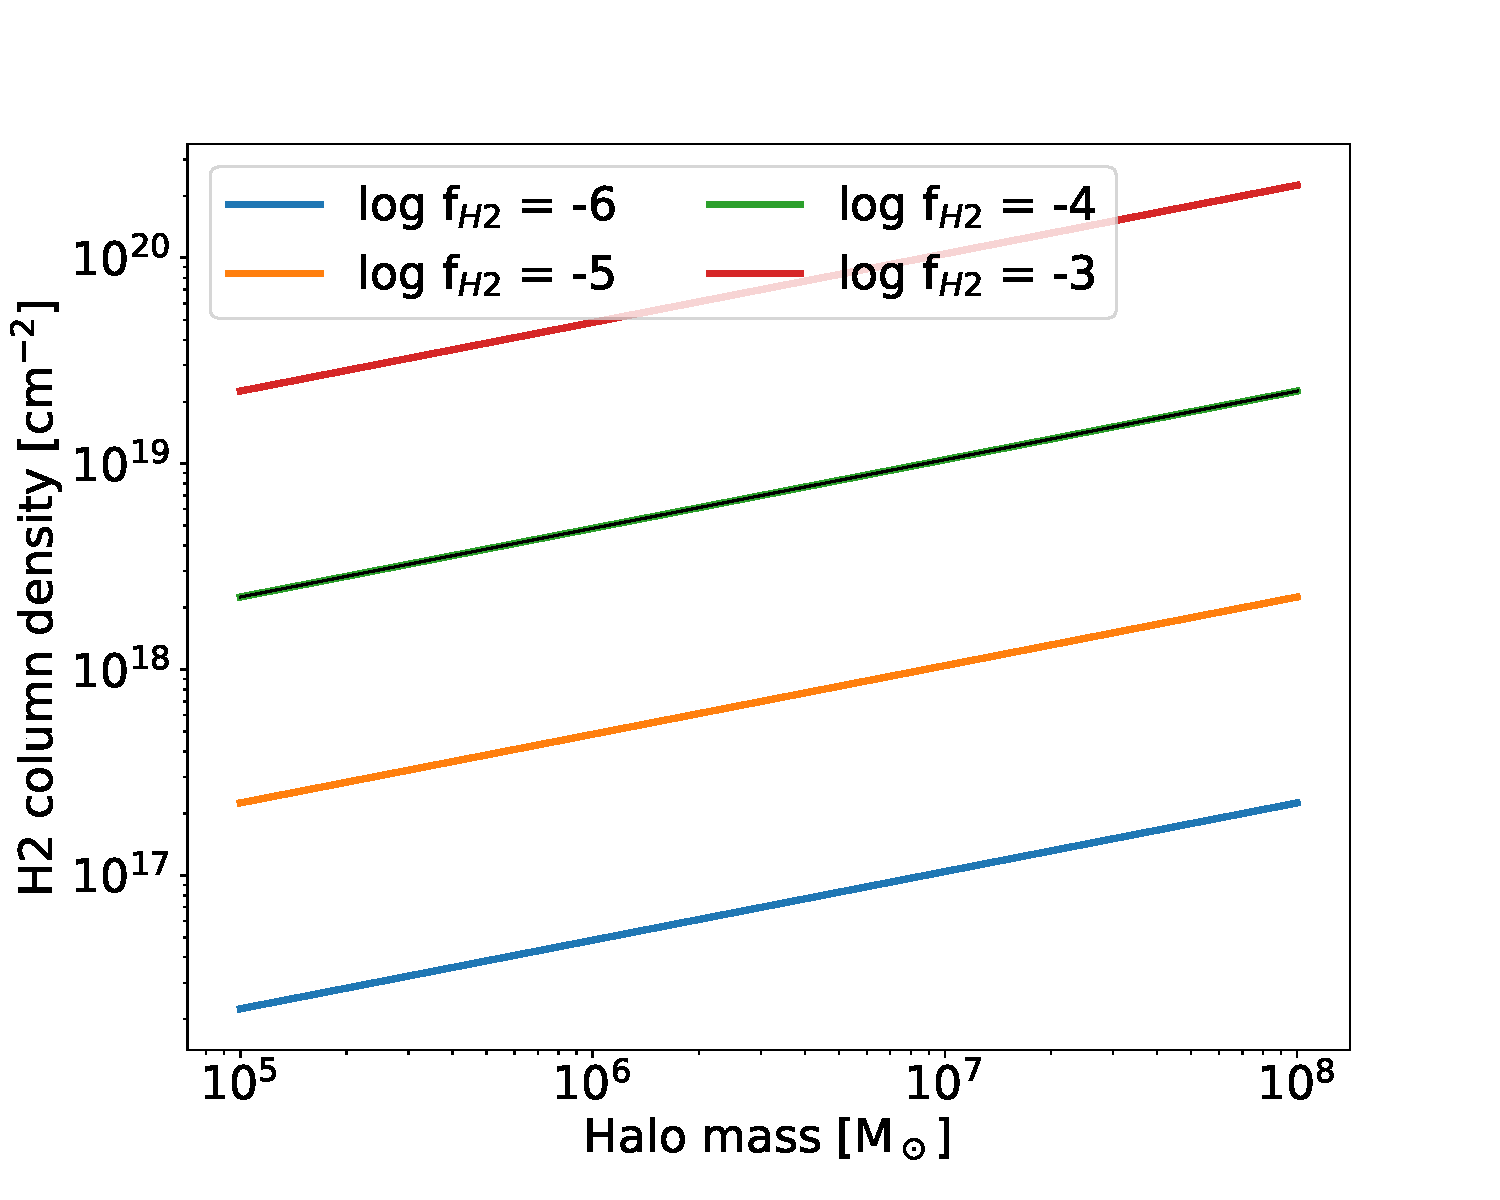
\includegraphics[width=\columnwidth]{images/H2_column_mass.pdf}
    \caption{\hh{} column density versus halo mass for varying shielding factors. At f$_{\rm H2}$ = $10^{-4}$, the shielding factor is equal to one and thus acts as the case where shielding is not applied to the halo.}
    \label{fig:H2_column_mass}
\end{figure}
%====================================================================
\section{Results}
%====================================================================
In this section, we will present the distribution of host halo masses of Pop III stars, the relation between the mass distribution and the LW background radiation, and the distribution of various Pop III properties.

To ensure that our box is representative of a typical piece of the universe, Figure \ref{fig:hmf} shows the simulated halo mass function along with the analytic Sheth-Tormen mass function at $z$ = 9.3. The analytic function closely matches our simulation until the mass resolution of our simulation is unable to resolve below 10$^{5}$ M$_{\odot}$ halos that contain $\approx$50 particles. 

\begin{figure}
	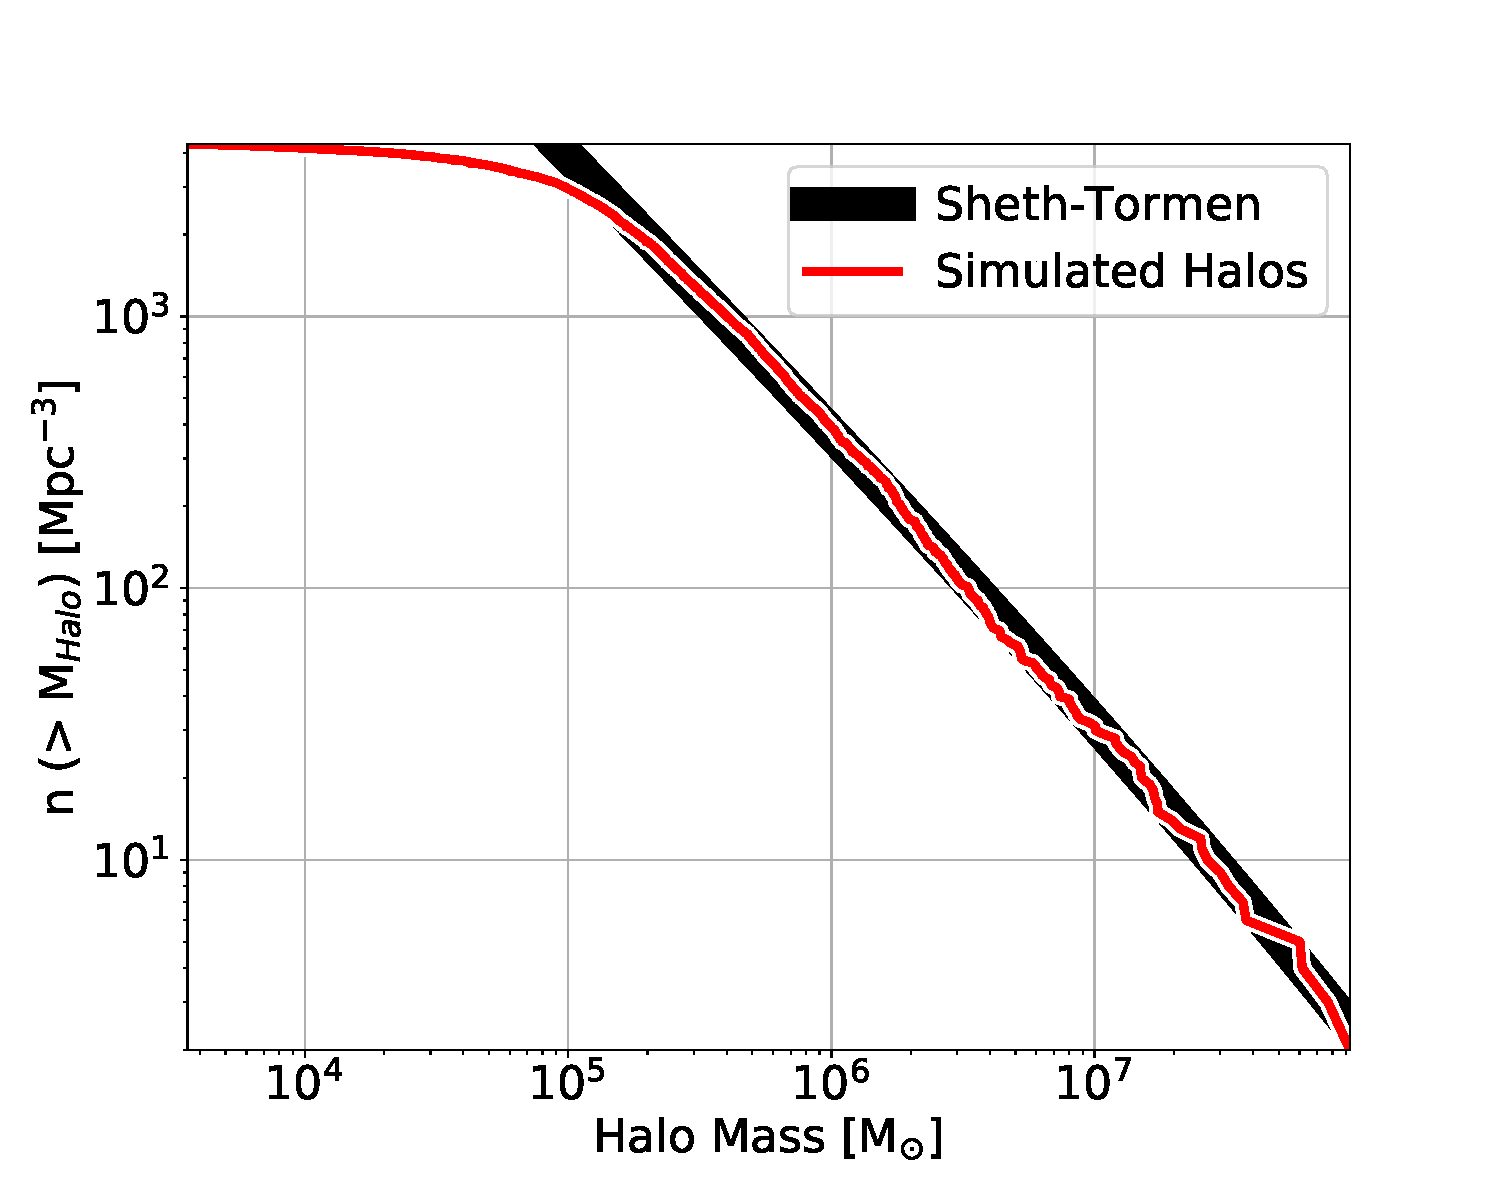
\includegraphics[width=\columnwidth]{images/hmf.pdf}
    \caption{Halo mass function of the last output of the simulation at $z$ = 9.3. The thick, black line is the analytic Sheth-Tormen mass function. The distribution of halo masses matches well with Sheth-Tormen until about 10$^{5}$ M$_{\odot}$.}
    \label{fig:hmf}
\end{figure}

As mentioned previously, Pop III stars form in our simulation only between 27.23 $\geq z \geq$ 9.39. During this time frame, a total of 688 Pop III stars form. The corresponding star formation rate density can be seen in Figure \ref{fig:pop3_SFR_bar}. Pop III star formation peaks at a redshift of 20 and slowly decreases. The star formation rate density does not fall to zero at the end of the simulation, since Pop III stars were still being produced when the simulation was cut off. The SFRD plotted here is particular for our box. Due to the small size of our box, we are unable to capture all of the cosmic variance. Therefore the SFRD is likely to change depending on the size and initial conditions of the box.

%====================================================================
\subsection{Population III host halo masses}
%====================================================================
 To determine the host halos of new Pop III stars, we use the halo finding code, \rockstar{} \citep{rockstar}. The mass determined by \rockstar{} is the dark matter mass, so to determine the total mass of the halos, we multiply the masses by $\Omega_{\rm M}$/$\Omega_{\rm DM}$. The total mass is subsequently used in our analysis. We also take the center and virial radius from the \rockstar{} halo catalog. A small percentage of Pop III stars do not form in a halo identified by \rockstar{}. Assuming that Pop III stars must form in collapsed halos, we calculate the virial mass and radius of a halo centered on the Pop III star directly from the simulation data. We calculate the LW intensity impinging on each halo by summing up the contribution coming from each radiating star particle outside the virial radius of the host halo. This is then added to the constant LW background implemented in the simulation (Eq. \ref{LWbg}). 

\begin{figure}
	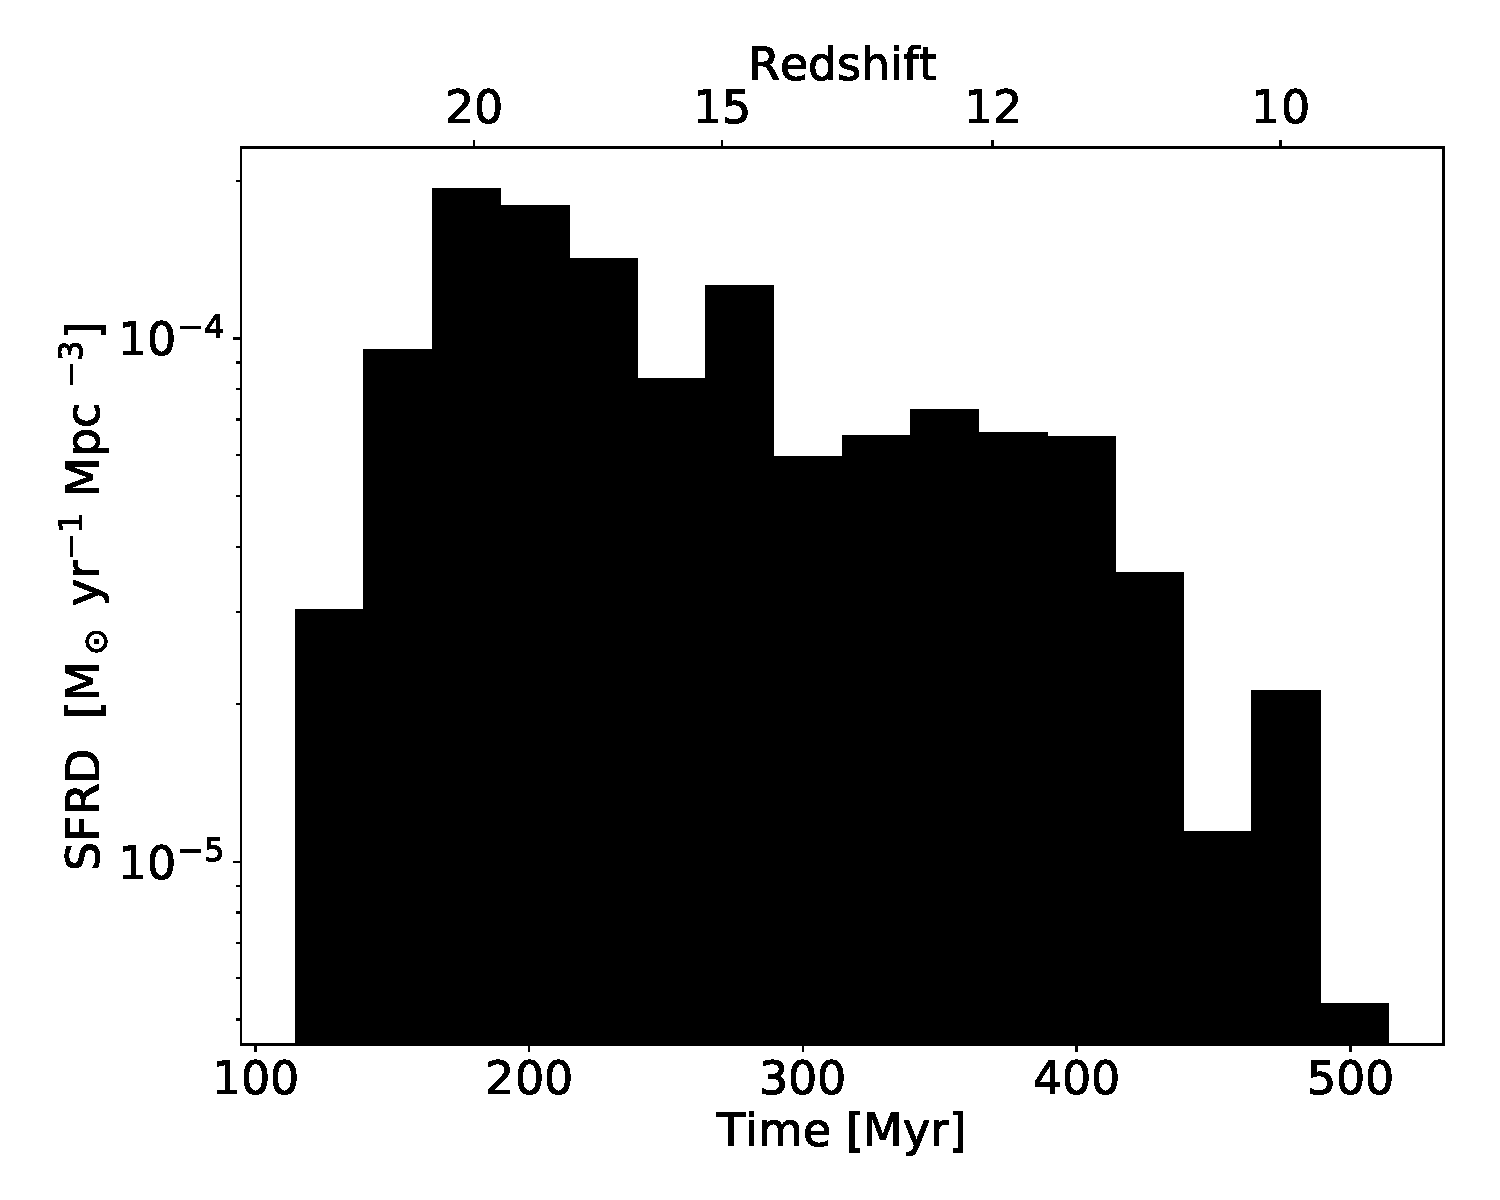
\includegraphics[width=\columnwidth]{images/pop3_SFR_bar.pdf}
    \caption{The star formation rate density of Pop III stars. It peaks at a redshift of 20, and slowly falls off. Note that metal-enriched star formation continually increases throughout time, although that is not plotted here.}
    \label{fig:pop3_SFR_bar}
\end{figure}

In redshift bins of $\Delta z$ = 1, the mean halo mass hosting Pop III stars is determined, and plotted as black dots against the redshift bins in Figure \ref{fig:mean_mass}. The median for each bin is by an x, and the 15.9\% and 84.1\% are plotted below and above the mean, respectively. The M01 relation (Equation \ref{mthresh}) for our LW background intensity in Eq. \ref{LWbg} is shown as the black solid line. Notably, the mean halo mass falls well below the relation, at 10$^{5.9}$ M$_{\odot}$ until $z$ = 11.5, at which point, the mean halo mass rises to 10$^{6.6}$ M$_{\odot}$. The large discrepancy between our data and the mass threshold from M01 is indicative of the \hh{} shielding which is included in our simulation. \hh{} shielding allows for halos to form at much lower masses, and therefore, Pop III stars are forming in these halos at earlier times. In the M01 analysis, \hh{} shielding is neglected in their calculations for a variety of reasons, including the Doppler broadening of LW bands and large column densities of \hh{} only beginning to form at late times. Interestingly, a full radiative transfer simulation, such as ours, does not produce identical results as M01 predicts. Throughout the literature, there appears to be a consensus that \hh{} self-shielding will help smaller mass halos collapse in the presence of a LW background radiation \citep[E.g.][]{Yoshida03, Ricotti01, Glover01, Hartwig15}. As can be seen by the red solid line in \ref{fig:mean_mass}, nearly 100\% of the halos hosting Pop III stars fall below the M01 relation, until around a redshift of 15, at which point, the mean halo mass begins to rise above the relation. The increase in the mean halo mass above the M01 relation is indicative of the increased LW intensity permeating the box due to a galaxy that becomes very active in star formation at late times. This galaxy has a halo mass of $10^{8.5} M_{\odot}$, a total stellar mass of $10^{6.5} M_{\odot}$, and has a peak Pop III SFR of $10^{-3.5} M_{\odot} yr^{-1}$ at $\approx$ 250 Myr and a peak metal enriched SFR of $10^{-1.3}$ at $\approx$ 500 Myr. This galaxy produces a large amount of LW radiation which dominates the box, and drives up the minimum halo mass required for the formation of Pop III stars. This increase in the LW background can also be seen in Figure \ref{fig:JLW_xe_mass}, where by the end of the simulation, the LW background rises to greater than 1 $J_{21}$.

\begin{figure}
	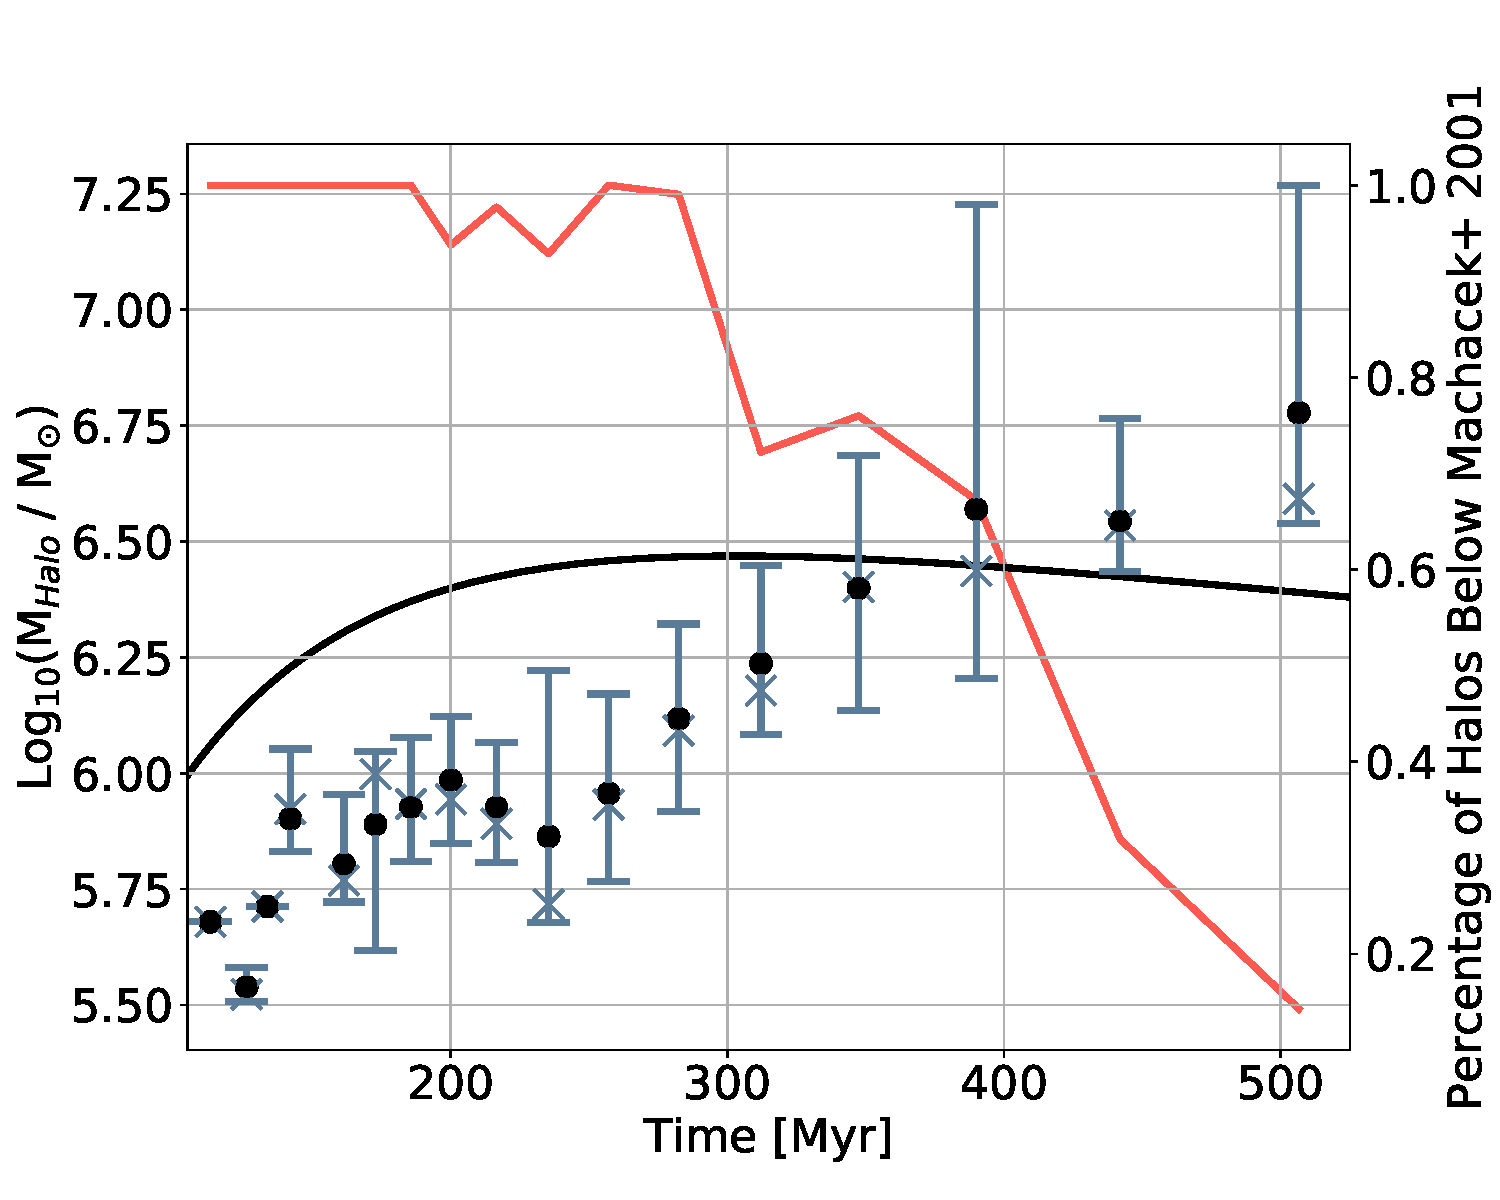
\includegraphics[width=\columnwidth]{images/mean_mass_errorb_fix.pdf}
    \caption{For halos hosting new Pop III stars, the mean halo mass for redshift bins of $\Delta z$ = 1 is plotted along the left hand side versus redshift. The black scatter points indicate the mean halo mass for that redshift bin and the x indicate the median halo mass. The error bars indicate the 15.9\% and 84.1\% percentiles. Plotted along the right hand side is the percentage of halos that fall below the M01 mass threshold, also plotted along redshift. The M01 mass threshold (Eq. \ref{mthresh}), is plotted for the constant LW background in Eq. \ref{LWbg}. Almost all halos fall below the M01 relation, until $z$ = 11.5, when the mean halo mass rises above the relation.}
    \label{fig:mean_mass}
\end{figure}

\begin{figure}
	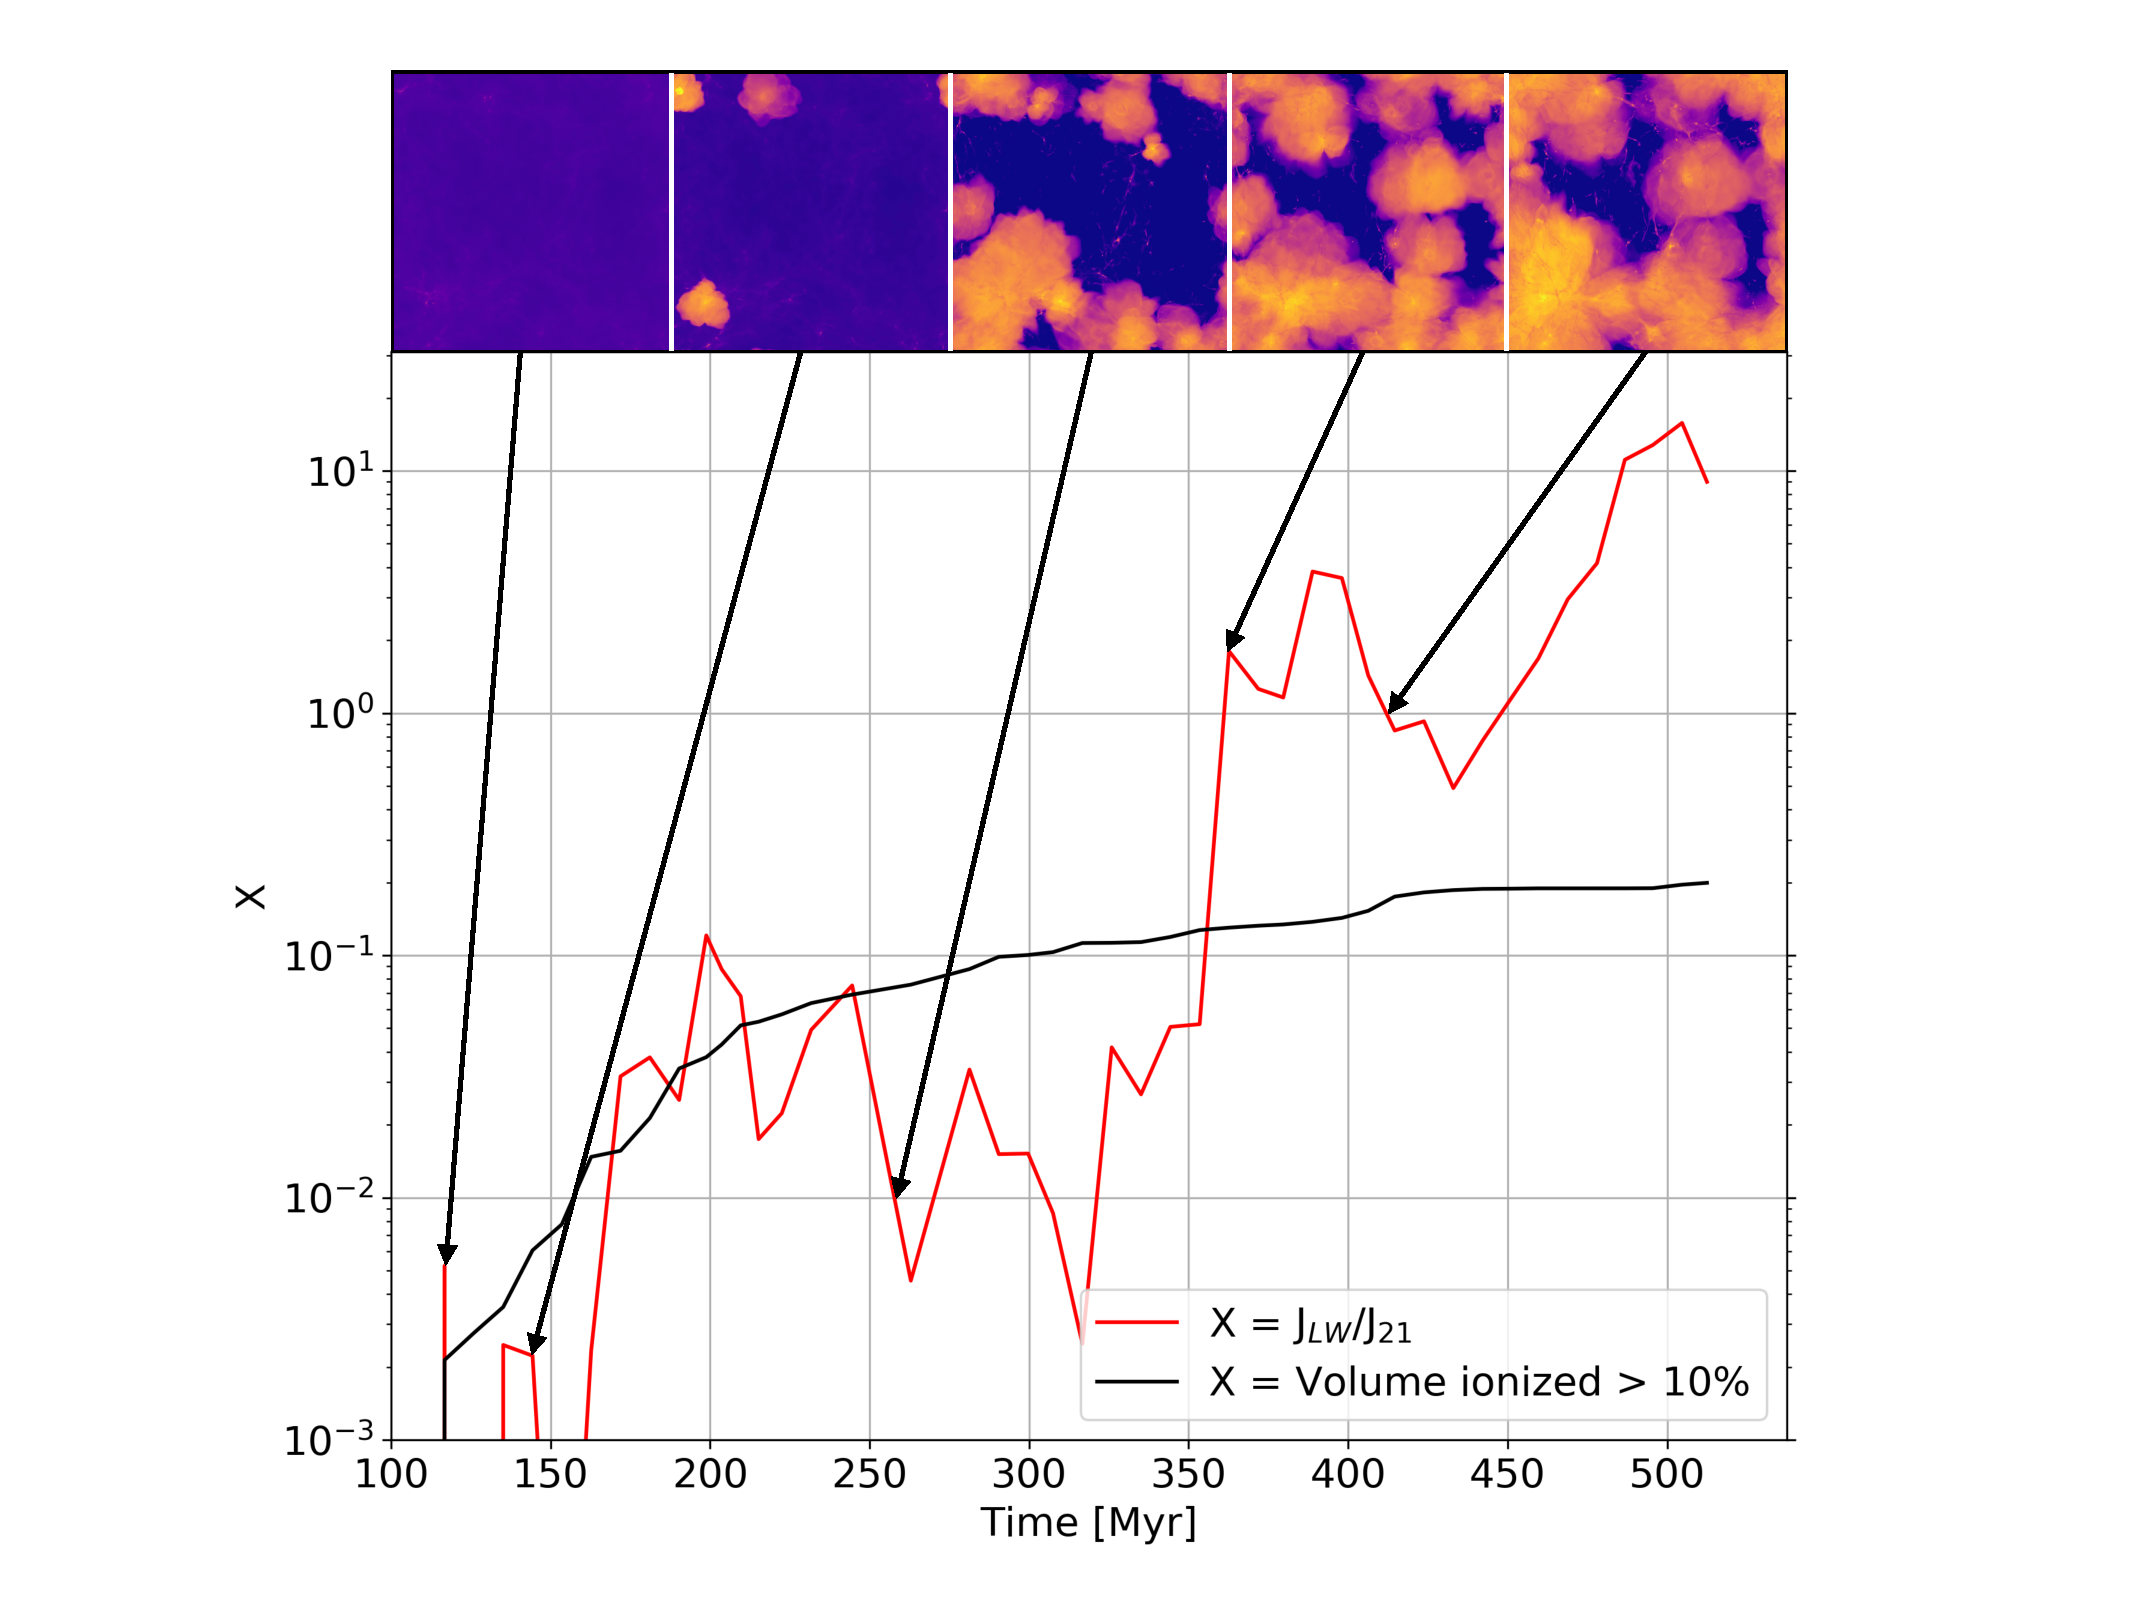
\includegraphics[width=\columnwidth]{images/JLW_xe_mass.pdf}
    \caption{For the entire box, the average mass weighted LW background and the fraction of the volume ionized above 10\% versus time. Temperature projections are shown at the points indicated by the arrows.}
    \label{fig:JLW_xe_mass}
\end{figure}

The LW background intensity versus the host halo mass for each Pop III halo in our dataset is shown in Figure \ref{fig:jlw_mass_machacek}. Each point is colored by the redshift where the Pop III star forms and the mass threshold from M01 (Eq. \ref{mthresh}) for the given LW background (Eq. \ref{LWbg}) is the solid black line. We see again that almost all halos form Pop III stars below the M01 threshold. There are also a few halos that form Pop III stars in very high J$_{\rm LW}$, below the relation. This situation arises when there are multiple Pop III stars forming at about the same time, within $\approx$ 100 pc of each other. Star formation can occur in a neighboring halo of a Pop III star whose LW radiation does not have ample time to photodissociate enough \hh{} to completely suppress star formation. The high J$_{\rm LW}$ is generally an indicator that the halos will likely have their star formation suppressed, but in cases where Pop III star formation occurs synchronically, star formation will not be suppressed, so long as they are a suitable distance away from each other. As there are only a few data points in this region, this situation is rare. It should be noted that there are duplicate halos within this plot, since halos are allowed to form multiple Pop III stars if the conditions are sufficient and each point represents an instance of Pop III formation. The grouped points in the higher end of J$_{\rm LW}$ are representative of such halos. We find that a total of 84\% of the halos forming Pop III stars lie below the M01 mass threshold over the entire simulation redshift range. We also do not see a clear relationship between the LW intensity and the host halo mass. This may be showing that the LW intensity is not as great an indicator of which halo will be allowed to for a Pop III star as previously thought. 

%====================================================================
\subsection{Multiple stellar systems}
%====================================================================

We now inspect the number of Pop III stars and the total mass of Pop III stars per halo. Again, we are only tracking massive stars, not any stars that may form out of fragmented gas with masses < $1 M_{\odot}$. Figure \ref{fig:totnump3_halomass_sidehist} shows the number of Pop III stars per halo for a given halo mass, just after star formation. The histogram of the number of Pop III stars for all masses is projected on the right hand side. We find that a median number of four Pop III stars form per halo, with a maximum of 16 Pop III stars forming per halo. Since we did not restrict the number of Pop III stars that can form in a halo, we find that the conditions are often sufficient for multiple Pop III stars to form in a single halo. Out of the halos forming Pop III stars, only 16\% of them form single Pop III stars, whereas 54\% form between two and five Pop III stars. It should be noted that these halos aren't necessarily forming all of the Pop III stars at once. For example, a halo can form stars again if it din't host a supernova. The number of Pop III stars that form within a halo is indicative of the star formation history of that halo. At the end of the simulation, Figure \ref{fig:final_redshift_Np3_mass} shows the distribution of the number of Pop III stars per halo for a given halo mass, for all halos in the simulation that host either a living or a remnant Pop III star. The red line shows the median number of Pop III stars for each halo mass bin. Figure \ref{fig:totp3mass_halomass_sidehist} shows the total mass of Pop III stars per halo for a given halo mass, where the histogram of the total Pop III mass for all halos is projected on the right hand side. Lines of constant star formation efficiency are overplotted. We find that most of our Pop III stars are forming between 10$^{-4}$ < f$_\star$ < 10$^{-3}$. The mean total mass of Pop III stars for all halos is 195 M$_{\odot}$.  


\begin{figure}
	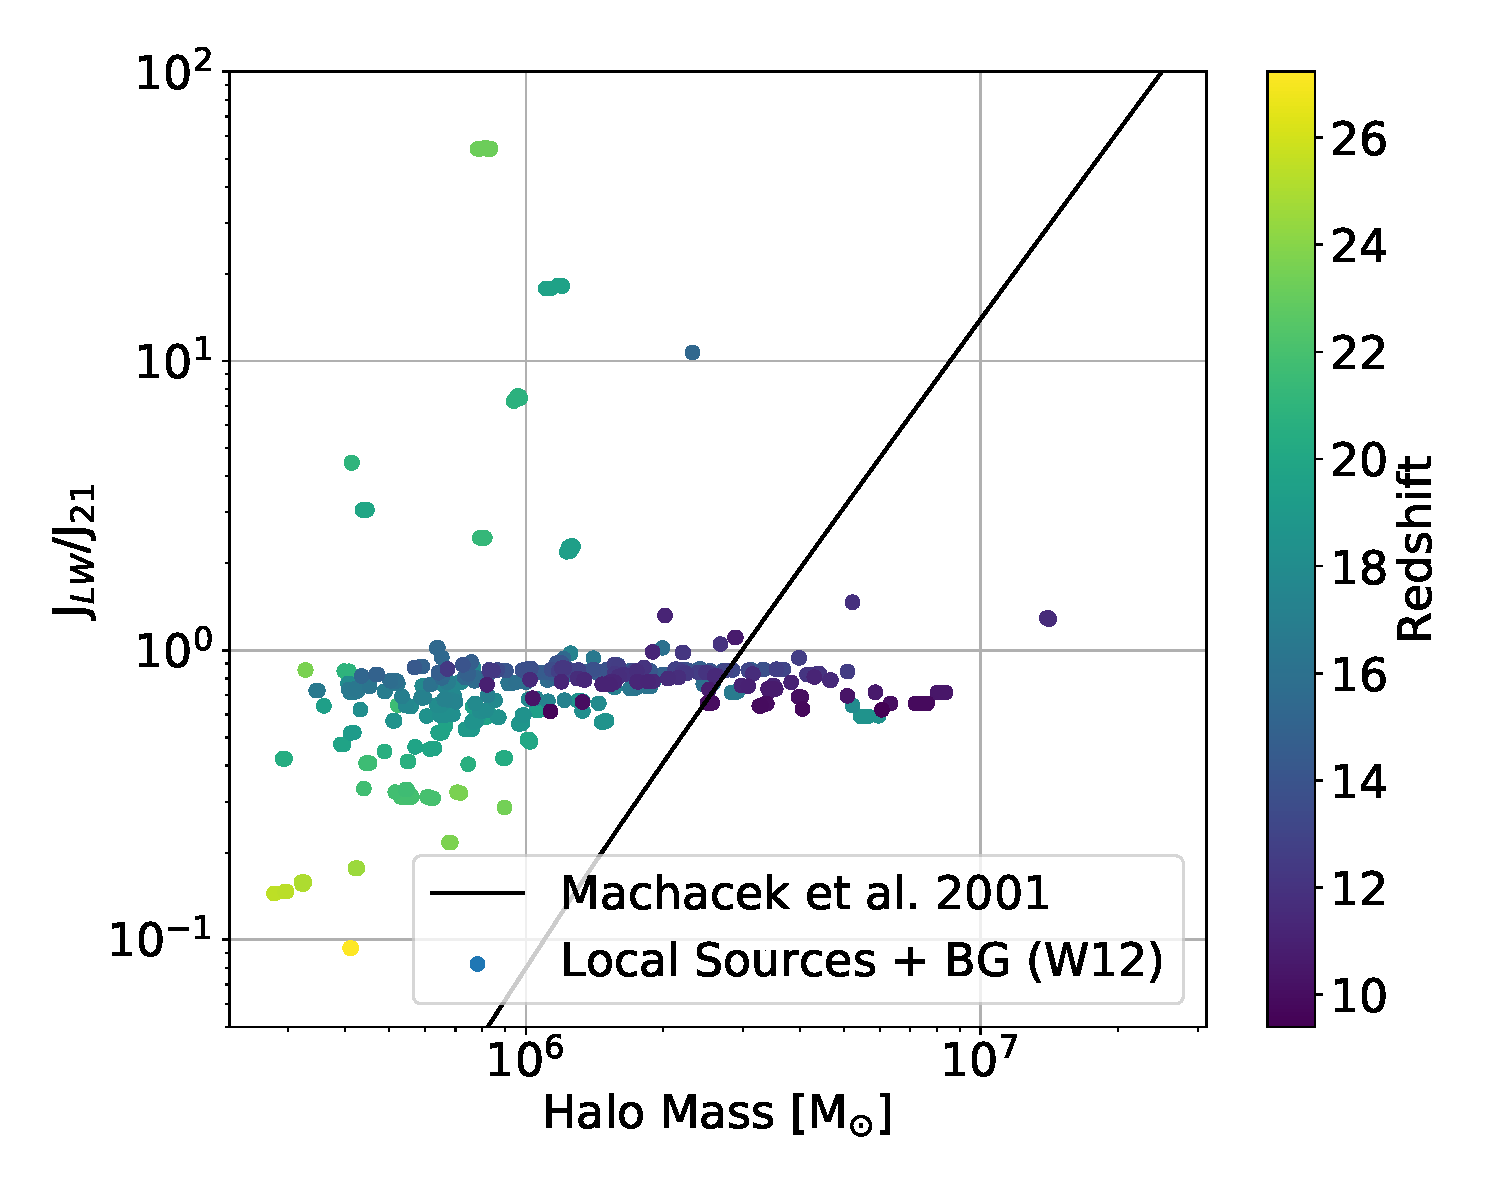
\includegraphics[width=\columnwidth]{images/jlw_mass_machacek_total.pdf}
    \caption{The average LW background for host halos of new Pop III stars is plotted versus the host halo mass, colored by redshift. The Machacek et al. relation is plotted given the background LW in Eq. \ref{LWbg}. Almost all halos fall below the relation, across a range of redshifts. A few halos (or possibly a single halo) allow Pop III stars to form at a low halo mass in a very high LW background. There are a few halos that have Pop III stars forming at later times and at high halo masses.}
    \label{fig:jlw_mass_machacek}{}
\end{figure}

\begin{figure}
	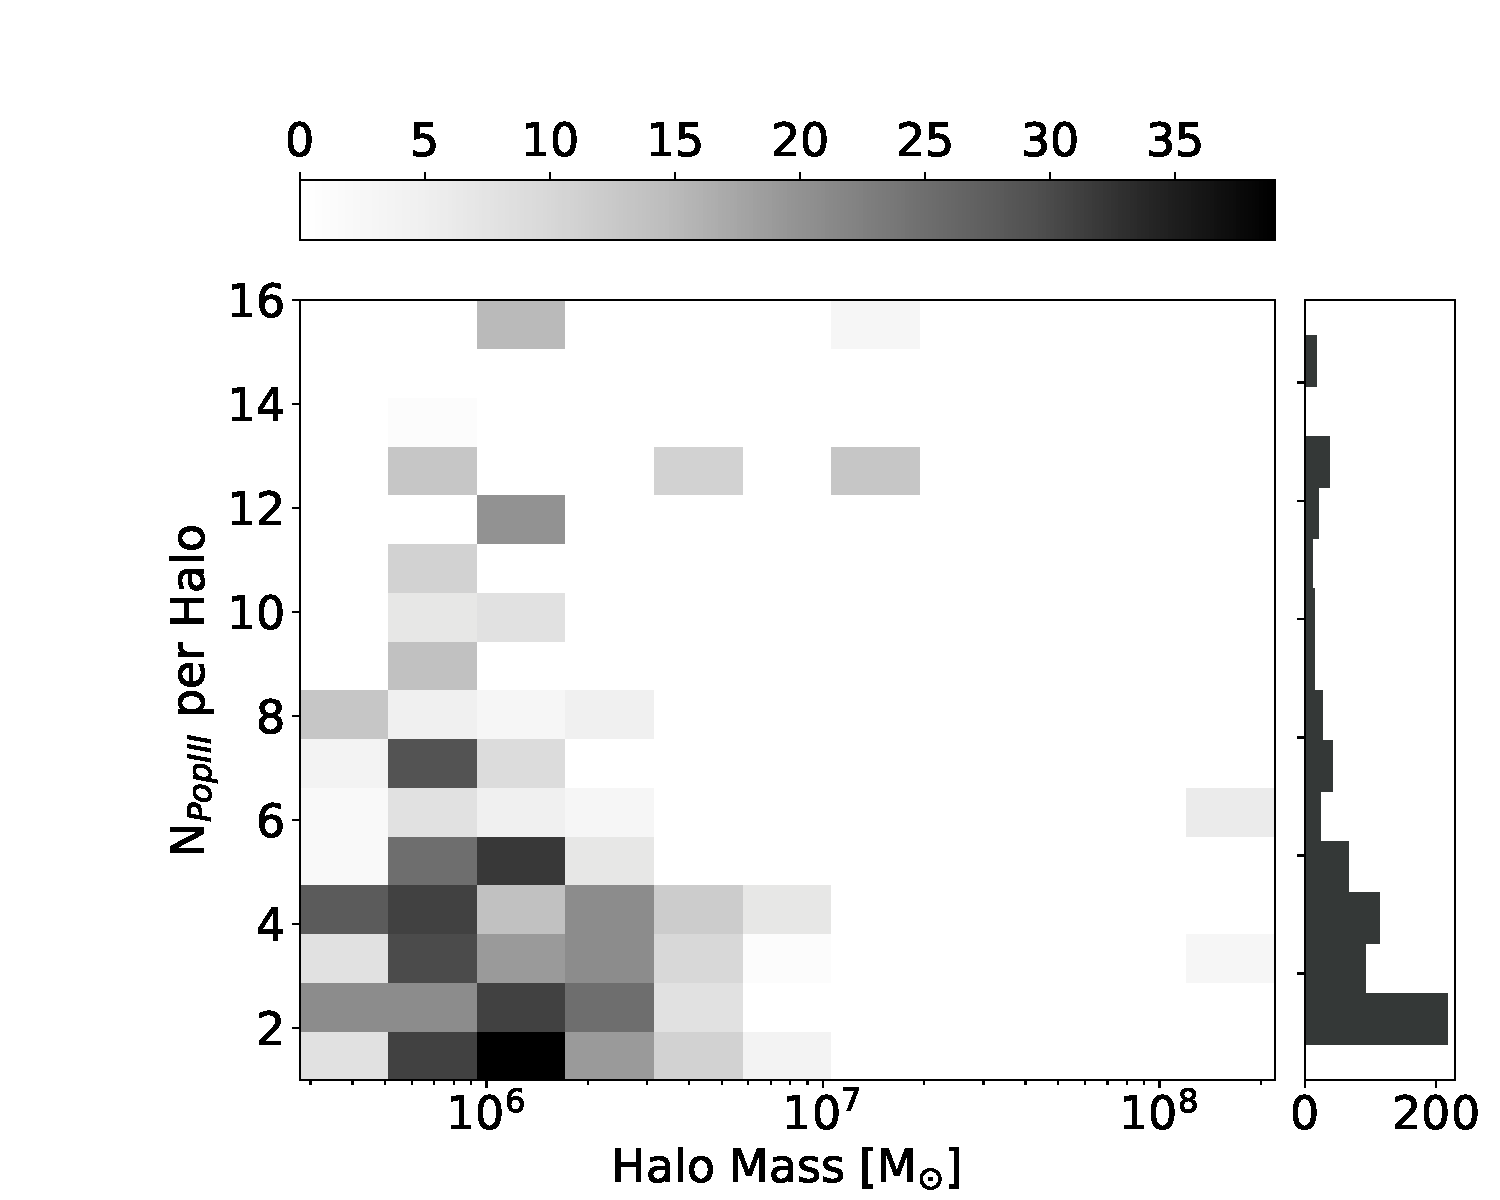
\includegraphics[width=\columnwidth]{images/totnump3_halomass_sidehist.pdf}
    \caption{Total number of Pop III stars in halos hosting new Pop III stars versus halo mass. A median number of four Pop III stars form in a single halo, with some forming as many as 16 Pop III stars.}
    \label{fig:totnump3_halomass_sidehist}
\end{figure}

\begin{figure}
	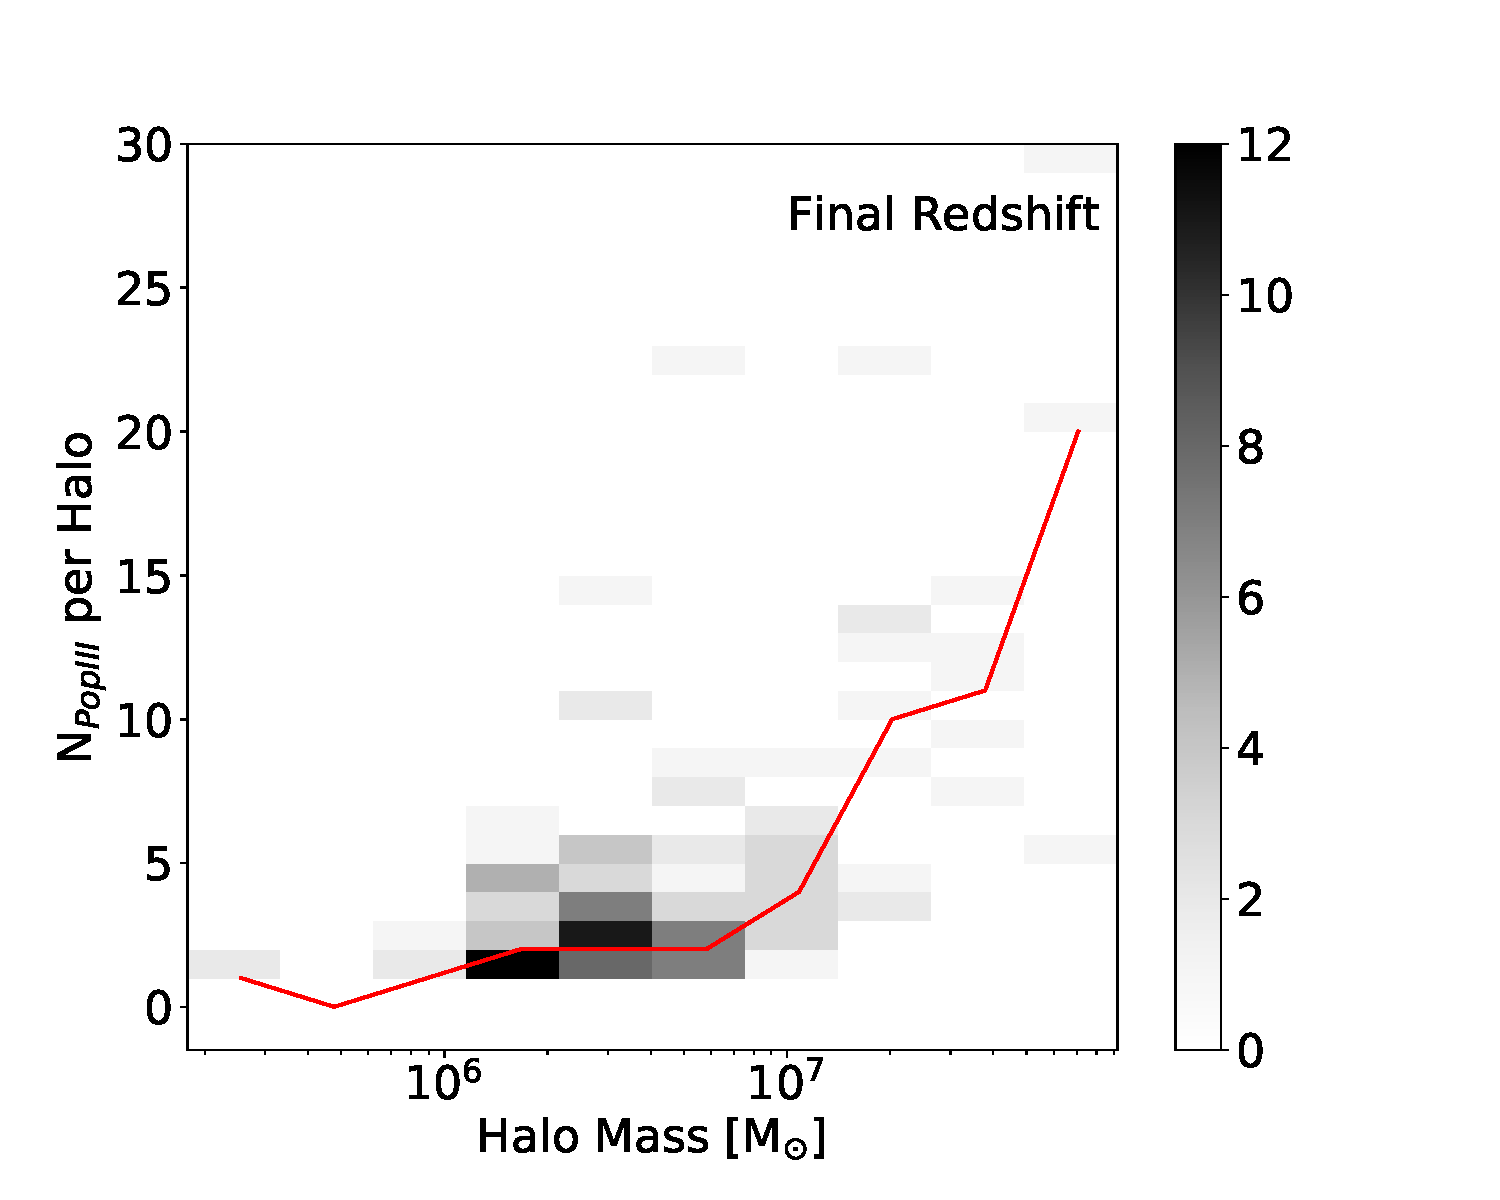
\includegraphics[width=\columnwidth]{images/final_redshift_Np3_mass.pdf}
    \caption{Total number of Pop III stars in all halos versus halo mass at the end of the simulation, at $z = 9$. The red line indicates the median number of Pop III stars in each halo mass bin.}
    \label{fig:final_redshift_Np3_mass}
\end{figure}

\begin{figure}
	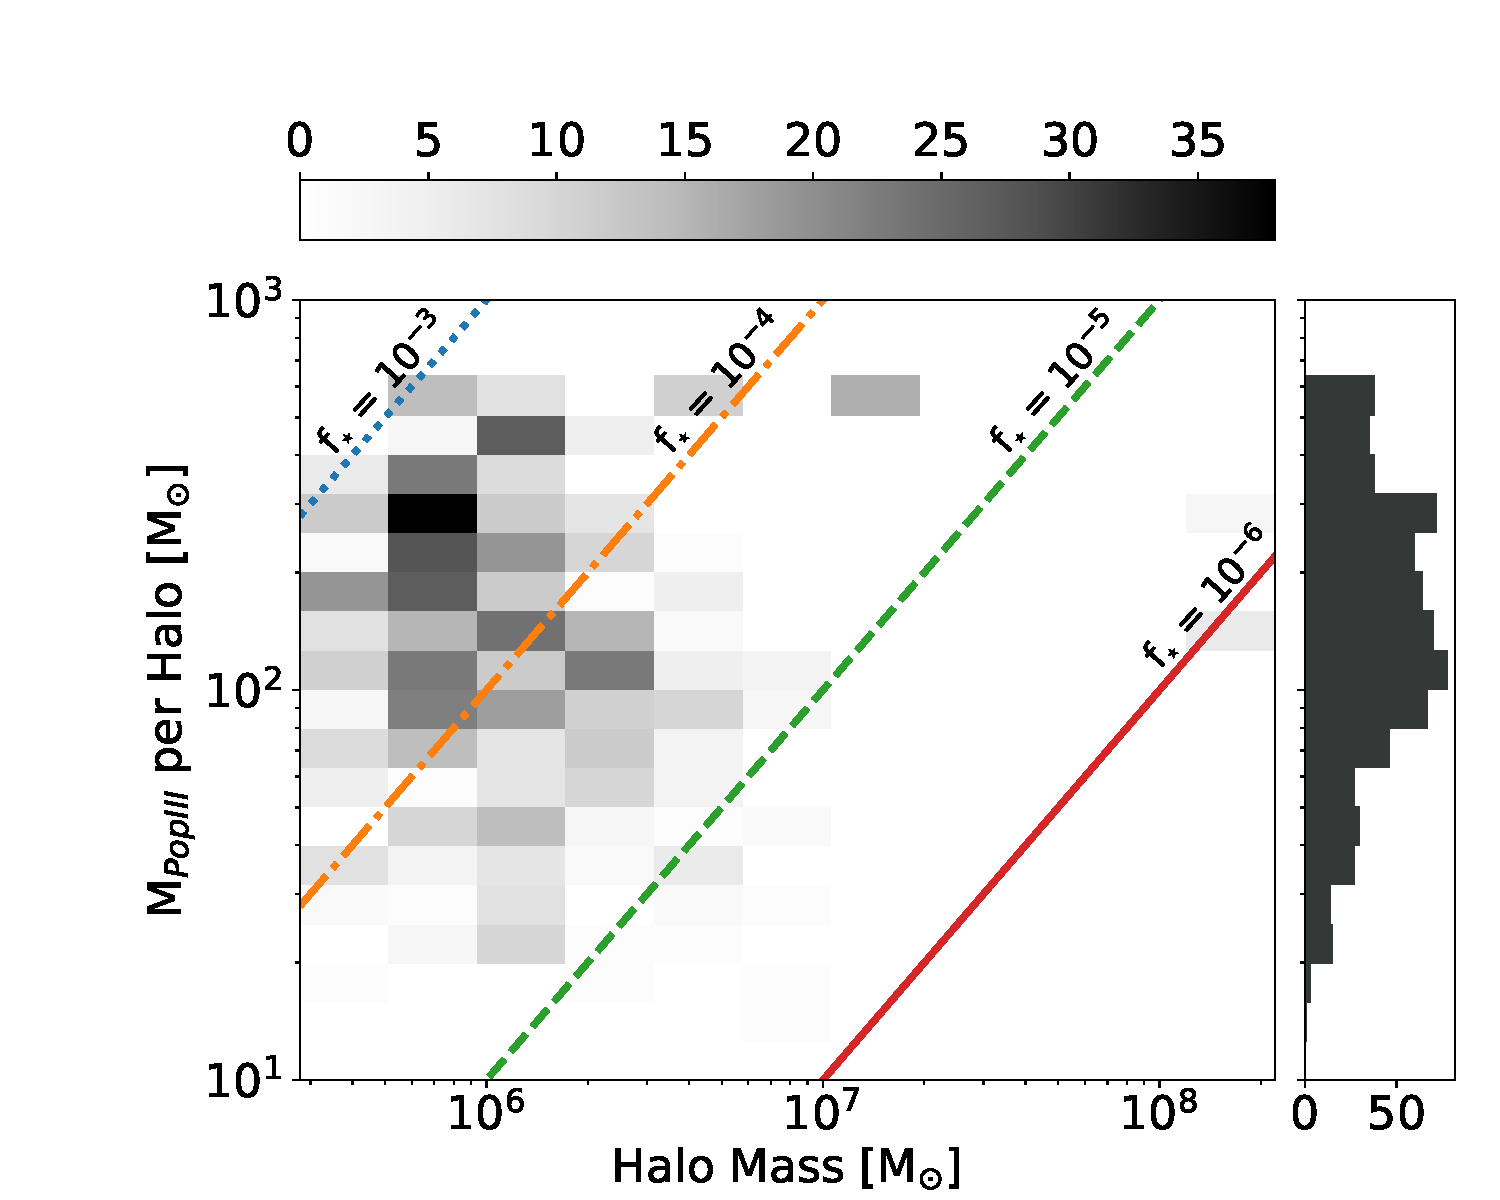
\includegraphics[width=\columnwidth]{images/totp3mass_halomass_sidehist.pdf}
    \caption{Total mass of Pop III stars in halos hosting new Pop III stars versus halo mass. Lines of constant star formation efficiencies are overplotted. Most halos form Pop III stars at efficiencies between 10$^{-3}$ and 10$^{-4}$.}
    \label{fig:totp3mass_halomass_sidehist}
\end{figure}

%====================================================================
\section{Discussion}
%====================================================================

%====================================================================
\subsection{Variations in the halo masses at collapse}
%====================================================================
Previous studies have focused on the minimum halo mass of Pop III hosts as a function of LW intensity. Pop III stars often form in halos up to an order of magnitude greater than the mininum. We also have found that Pop III star formation occurs in a similar range of host halo masses throughout our simulation. There are three main causes of this significant variation in mass. First, a fraction of metal-free stars directly form a black hole without metal ejecta \citep{Heger03}, leaving the halo chemically pristine.  Second-generation stars forming later in that halo could still be metal-free if no external enrichment occurs. Thus they would form in halos substantially larger than the minimum, as it takes tens of millions of years for the halo to recover its gas after radiative feedback \citep{Muratov13, Jeon14_Recovery}.  Second, dynamical heating from mergers and accretion provide a heating source inside the growing halo, preventing the gas from efficiently cooling via \hh{}. This turbulent stirring can delay star formation that could cool through \hh{} in an ideal situtation but otherwise forms in halos more massive than the minimum \citep{Yoshida03, Wise19}. Finally, temporal fluctuations in the local LW radiation field can greatly affect the amount of \hh{} within a halo and thus, how efficiently the halo can cool. While this may only be a small effect in some halos where the local LW radiation flucutations are relatively small and star formation is distant, Pop III star formation may be significantly delayed or completely prevented in halos that are close to active star formation sites.  In summary, the timing of Pop III star formation depends on both local -- halo histories of star formation and growth -- and environmental properties.  The combination of these three processes determines which halos will be able to form Pop III stars, and thus results in a wide range of host halo masses. 


%====================================================================
\subsection{Comparison to previous work}
%====================================================================

There has been a large amount of work done throughout the literature investigating the relationship between the LW background intensity and halo masses. \citet{Tegmark97} numerically integrated a chemical network to calculate the minimum mass a halo must have in order to cool, by considering \hh{} formation and cooling rates. They conclude that cooling by \hh{} is efficient and leads to the first formation of structures. They found a minimum halo mass needed to collapse which depends on the virial temperature of the halo and the virial redshift. At $z = 20$, this minimum halo mass is $4 \times 10^{6} M_{\odot}$. \citet{Trenti09} uses a similar argument as \citet{Tegmark97}, and found that metal-free halos can exist until z $\approx$ 6 using cosmological simulations and analytical calculations for metal enrichment. They also provide some insight into whether or not Pop III supernova rates are high enough within these metal-free halos to allow for the Large Synoptic Survey Telescope to see these regions of the universe. They used the minimum halo mass capable of cooling via \hh{} from \citet{Trenti09_SFR} as one part of their halo mass model (see the blue solid line in Figure \ref{fig:compare_JLW_mass}, given our LW background). Neither \citet{Trenti09} nor \citet{Tegmark97} included the effects of \hh{} self-shielding, which can explain the discrepancy between our data and their mass threshold relationship (Figure \ref{fig:compare_JLW_mass}). \citet{Mebane18} used a semi-analytic model of star formation, including feedback properties such as a LW background, photoionization due to Pop III stars, supernovae of Pop III stars and metal-enriched stars, and chemical enrichment, to determine for how long Pop III stars will survive for and found that Pop III stars can continue to form until z $\approx$ 6. They found a minimum halo mass for hosting Pop III star formation, but with the caveat that they did not include \hh{} self-shielding. They found that when Pop III stars contribute to the LW background, the minimum halo mass for Pop III star formation is $4 \times 10^{6} M_{\odot}$ as $z = 20$, similar to results from \citet{Tegmark97}. The results from \citet{Trenti09} and \citet{Mebane18} have higher halo masses in comparison with M01, although this more closely matches results from simulations (see \citet{Wise07_UVB, OShea08}). It should be noted that because our box is fairly small, we cannot capture the cosmic variance of rare halos and galaxies. For example, at late times, a single galaxy dominates the LW radiation field, and drives up the host halo masses. However, we would expect this to happen at different times in other cosmological volumes. Therefore, we cannot directly compare the time dependence, however, a comparison as a function of LW intensity is still valid. 

\citet{Yoshida03} used cosmological simulations to study the formation of primordial star-forming clouds. They followed the growth of structure to find where gas cools and condenses which would form the first stars, and how the effects of LW radiation may affect these gas clouds. Importantly, they included \hh{} self-shielding within halos. In a series of simulations, they found a minimum halo mass for those halos hosting gas clouds which may result in active star formation (see their Figure 12). They found that in the presence of a LW background of J$_{21}$ = 0.01, the minimum halo mass at $1.5 \times 10^{6} M_{\odot}$. When \hh{} self-shielding is taken into account along with a LW background, they see these halo masses decrease to $9 \times 10^{6} M_{\odot}$. This value lies close to the case where there is no LW background applied, where the minimum halo mass is $7 \times 10^{5} M_{\odot}$. They find that \hh{} self-shielding does appear to be an efficient mechanism for primordial gas cooling. In comparison with our work, we find similar minimum halo masses for each redshift, although we do see a wider range of halo masses across redshifts, ranging from 10$^{5.4}$ M$_{\odot}$ to 10$^{7.1}$ M$_{\odot}$. While our halos never experience a LW intensity as low as 0.01, we find that their minimum mass for this LW intensity lies in the same mass range as our halos (see blue open circle in Figure \ref{fig:compare_JLW_mass}) (this may change !!! ). \citet{Wise07_UVB} used cosmological simulations to investigate \hh{} cooling in a LW background. They found that \hh{} cooling is dominant even when there is a large LW background present. They included dynamical heating but did not include self-shielding, and subsequently found halo masses at their collapse that lie well above the M01 relation (see red open triangles in Figure \ref{fig:compare_JLW_mass}). Their J$_{LW}$ = 0 control is plotted in Figure \ref{fig:compare_JLW_mass} at J$_{LW}$/J$_{21}$ = 10$^{-4}$. \citet{OShea08} used cosmological simulations to investivate Pop III star formation in various LW backgrounds. They found that due to an increased LW background, there is a delay in star formation, and thus there is an increase in the halo masses at collapse. They also ignored \hh{} self-shielding in their calculations and included dynamical heating, which can again account for the increased halo masses they found compared to this work, as can be seen in Figure \ref{fig:compare_JLW_mass} (open green squares). Their halo masses are similar to the results of \citet{Wise07_UVB}. Their control of J$_{21}$ = 0 control is plotted at J$_{LW}$/J$_{21}$ = 10$^{-4}$.

\begin{figure}
	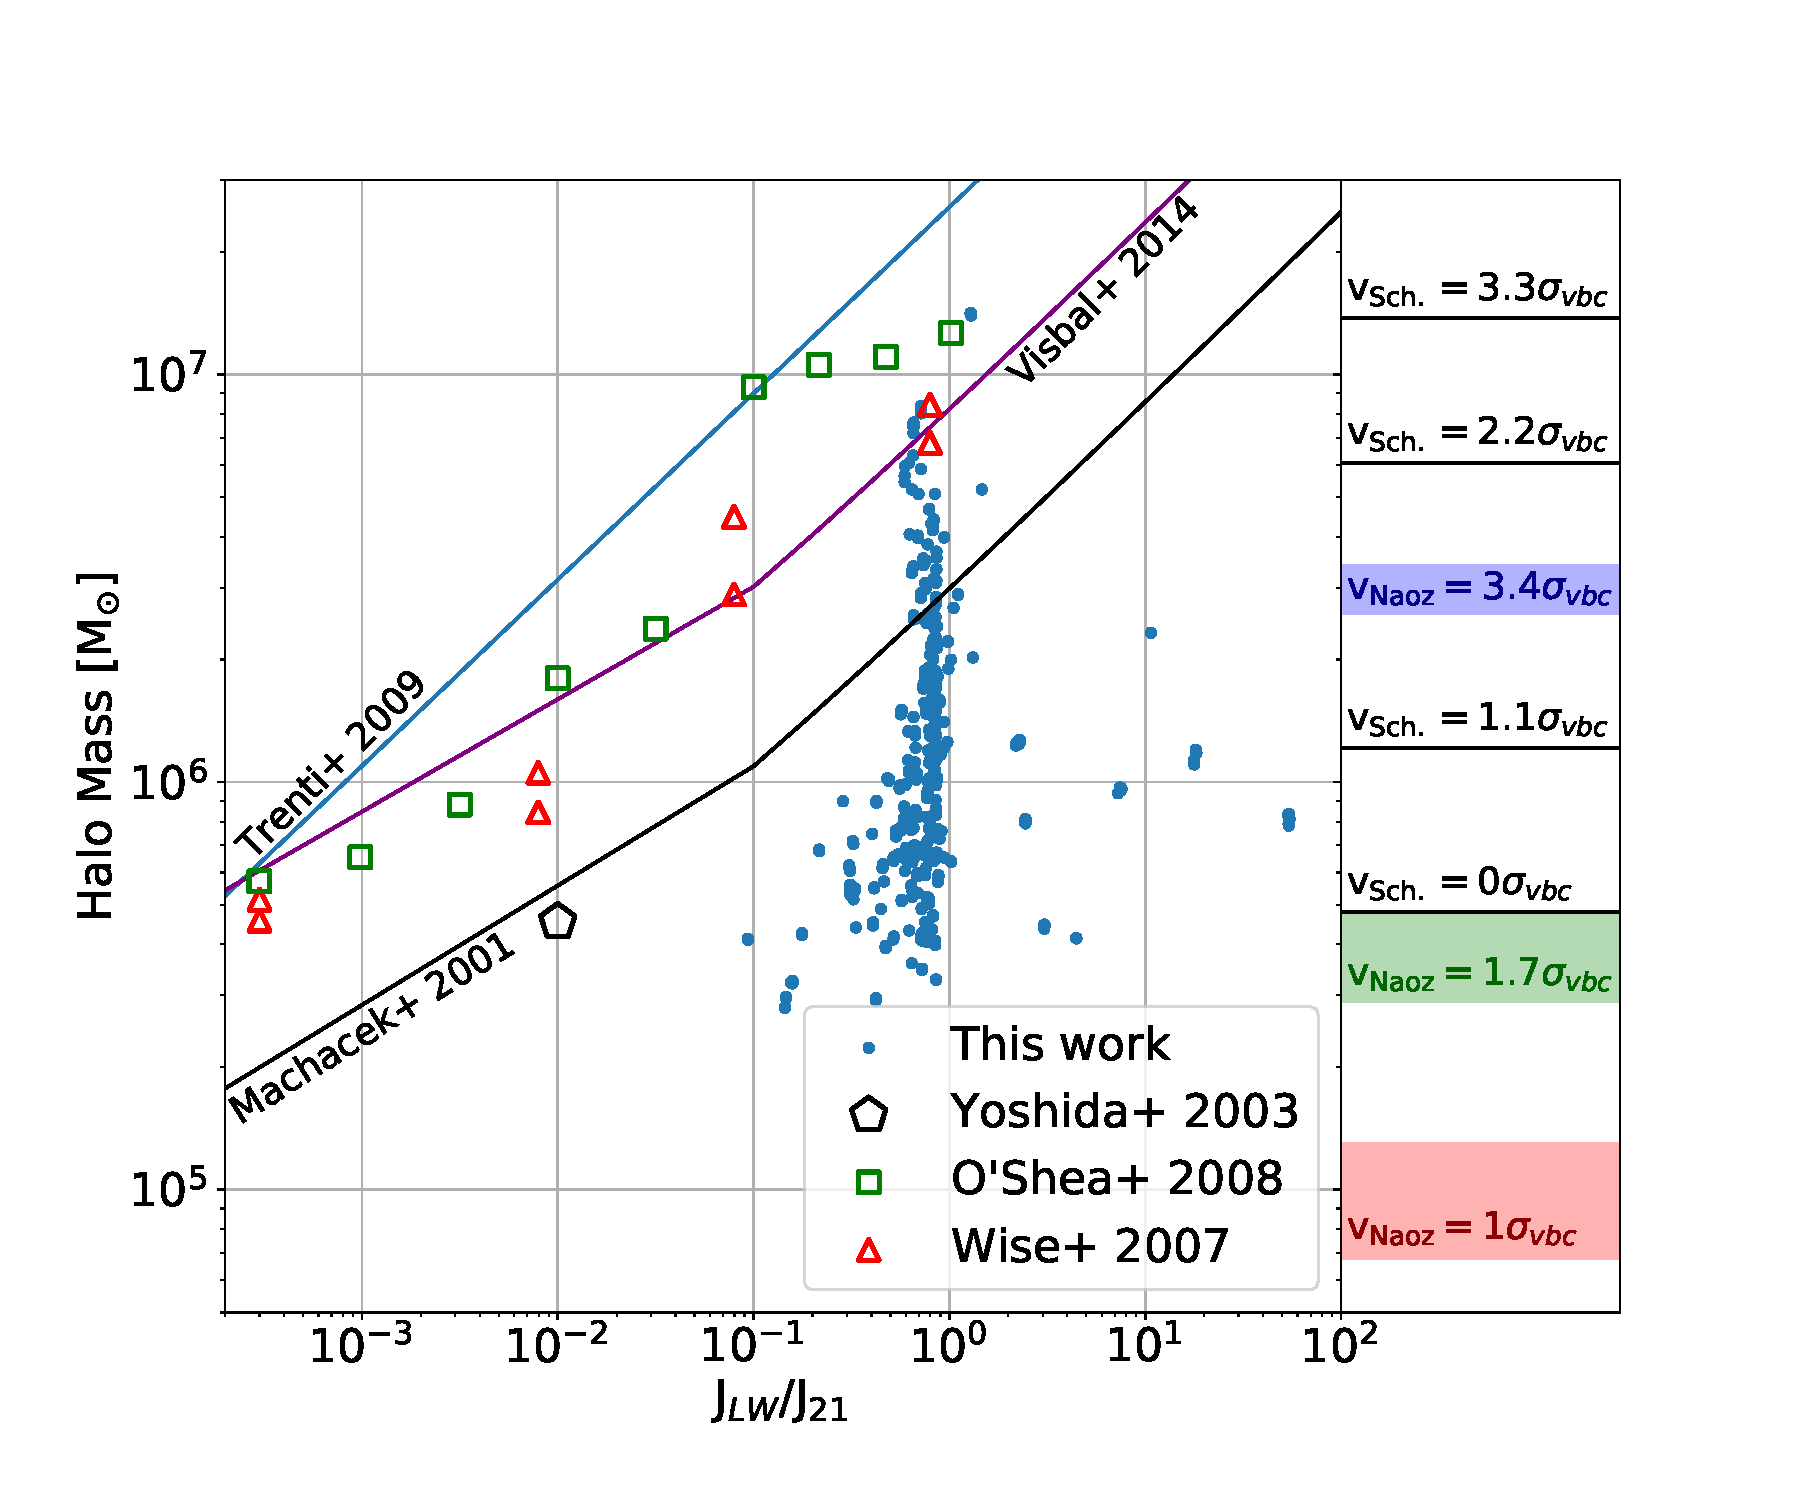
\includegraphics[width=\columnwidth]{images/compare_JLW_mass.pdf}
    \caption{The average LW intensity normalized by J21 versus the halo mass for this work and a variety of other works. The black solid line is from M01, blue solid line from \citet{Trenti09_SFR}, blue open circle from \citet{Yoshida03}, green open squares from \citet{OShea08}, and red open triangles from \citet{Wise07_UVB}. J$_{LW}$ = 0 for the various sources is plotted here at J$_{LW}$/J$_{21}$ = 10$^{-4}$. The solid bands of halo masses correspond to the characteristic masses of halos to contain a baryon fraction that is half of the cosmic mean for various redshifts and for the shown streaming velocities from \citet{Naoz13}. For each band, the maximum halo mass occurs at $z = 15$. For streaming velocities of $3.4 \sigma_{\rm vbc}$, $1.7 \sigma_{\rm vbc}$, and $1 \sigma_{\rm vbc}$, the minimum halo mass occurs at $z = 17, 22, \rm{and} \ 27$, respectively.}
    \label{fig:compare_JLW_mass}
\end{figure}

%====================================================================
\subsection{Caveats}
%====================================================================

There are a few minor shortenings to this work that should be noted. \citet{Schauer17} investigated the escape fraction of LW photons in the near-and far-field and found that the LW escape fraction of atomic cooling halos can vary significantly depending on the ionisation front within the halo. In the near-field with an outbreaking ionisation front, they find that the LW escape fraction is greater than 95\%. But when the ionisation front is slowly moving, they found that the LW escape fraction can range from 3\% to 88\%. In general, they find that the LW escape fractions in the far-field are higher than 75\%. In our work, we allow all LW photons to escape the halo. Since we are not accounting for the reduced escape fraction within our halos, we are overestimatng the LW radiation coming from point sources in our simulation. We could account for this by decreasing the intensity of the stars, since the overall LW radiation would be reduced, although this should not significantly affect our results as we find little dependence on LW intensity. We also do not include streaming velocities between baryons and dark matter within our simulation \citep{Tselia11, Greif11_Delay, Naoz12, OLeary12}. Streaming velocities can suppress star formation at very high ($z \ga 20$) redshifts only, because the streaming velocities decrease with time. Pop III star formation is delayed by an average of $\delta z = 4$ by increasing the halo mass needed to overcome the bulk velocity by about a factor of three \citep{Greif11_Delay}. The streaming velocities will generally result in lower gas densities within halos as well as an offset of the peak density from the center of the halo \citep{OLeary12}. Often in the literature, streaming velocities are only studied for a few halos. But \citet{Naoz13} estimated the minimum mass needed to retain the bulk of the baryons within the dark matter halo using a series of cosmological simulations, the results of which can be seen in Figure \ref{fig:compare_JLW_mass} (see shaded bands). These halos only reach up to about $2 - 3 \times 10^5 M_\odot$ when the streaming velocity is about $1\sigma_{\rm vbc}$, which is smaller than the star forming halos in our simulation. \citet{Naoz13} mention that at the largest streaming velocity, their simulations do not match expected values due to a small sample size of high mass halos. If we had included streaming velocities, the gas would have already fallen into the dark matter potential well when the halo exceeds this characteristic mass. Because of this, streaming velocities would likely not affect our results. Finally, there is the obvious caveat of the unknown Pop III IMF. Like with any work done assuming a Pop III IMF, uncertainties about metal enrichment, multiplicity, total stellar mass, ionization rates, supernova rates, and the amount of black holes produced are introduced into our results.

%====================================================================
\section{Conclusions}
%====================================================================
In this work, we presented the analysis of the host halo mass distribution of Pop III stars and how it relates to the LW background radiation. We find that Pop III stars are forming in halos with a mean mass of $10^{5.9} M_\odot$ until $z = 11.5$, which falls well below the M01 relation due to \hh{} self-shielding. The mean halo mass then rises above the M01 to a mean value of $10^{6.6} M_\odot$ due to the domination of LW radiation throughout our simulation box produced by metal-enriched stars. As we compare with the literature, we appear to have much lower halo masses than those that do not include \hh{} self-shielding, so it appears that this is an important process that is often ignored in calculations. We also see that there doesn't appear to be a correlation between the average LW intensity with a halo and the halo mass. Therefore, the LW intensity may not be as indicative of which halos may form Pop III stars as previously thought. Pop III stars are often assumed to form in isolation, but we are finding that most of our halos are forming multiple Pop III stars, with a median number of four Pop III stars in a single halo, up to a maximum of 16 Pop III stars. 

%====================================================================
\section*{Acknowledgements}
%====================================================================

JHW is supported by National Science Foundation grants AST-1614333 and OAC-1835213, NASA grant NNX17AG23G, and Hubble theory grant
HST-AR-14326.  We thank the support staff at Georgia Tech's PACE,
where we ran this simulation.  The freely available plotting library
{\sc matplotlib} \citep{matplotlib} was used to construct numerous
plots within this paper. Computations and analysis described in this
work were performed using the publicly-available \enzo{} and \yt{}
codes, which is the product of a collaborative effort of many
independent scientists from numerous institutions around the world.

%%%%%%%%%%%%%%%%%%%%%%%%%%%%%%%%%%%%%%%%%%%%%%%%%%

%%%%%%%%%%%%%%%%%%%% REFERENCES %%%%%%%%%%%%%%%%%%

% The best way to enter references is to use BibTeX:

\bibliographystyle{mnras}
\bibliography{jwise} % if your bibtex file is called example.bib


% Alternatively you could enter them by hand, like this:
% This method is tedious and prone to error if you have lots of references
%\begin{thebibliography}{99}
%\end{thebibliography}

%%%%%%%%%%%%%%%%%%%%%%%%%%%%%%%%%%%%%%%%%%%%%%%%%%

%%%%%%%%%%%%%%%%% APPENDICES %%%%%%%%%%%%%%%%%%%%%

\appendix

%%%%%%%%%%%%%%%%%%%%%%%%%%%%%%%%%%%%%%%%%%%%%%%%%%


% Don't change these lines
\bsp	% typesetting comment
\label{lastpage}
\end{document}

% End of mnras_template.tex